\documentclass[11pt, oneside]{article}   	% use "amsart" instead of "article" for AMSLaTeX format
\usepackage{geometry}                		% See geometry.pdf to learn the layout options. There are lots.
\usepackage{xcolor}					% for doing text colors
\geometry{letterpaper}                   		% ... or a4paper or a5paper or ... 
%\geometry{landscape}                		% Activate for rotated page geometry
%\usepackage[parfill]{parskip}    		% Activate to begin paragraphs with an empty line rather than an indent
\usepackage{graphicx}				% Use pdf, png, jpg, or eps§ with pdflatex; use eps in DVI mode
								% TeX will automatically convert eps --> pdf in pdflatex		
\usepackage{amssymb, amsmath}
\usepackage{caption, subcaption}


% Tracking changes: see https://jansoehlke.com/2010/06/strikethrough-in-latex/ for strikethroughs in latex
\usepackage[normalem]{ulem} % for horizontal strike throughs

\usepackage{tikz, pgfplots} 					% For diagrams
\usetikzlibrary{shapes, arrows.meta, % arrows.meta lets me do other arrow head types like square, 			
			quotes, trees,		%see https://gist.github.com/AndiH/f99d9b0cbd3519c27af5b96cfbeff97c
			calc} 	
\usepackage[shortlabels]{enumitem} % so I can have an enumerated list going H1, H2, ...	
\pgfplotsset{mystyle/.append style={axis x line = bottom, axis y line = left, xlabel = {$x_i$}, ylabel = {$\sigma_i(x_i)$}}}

% Allows theorems and proofs
\usepackage{amsthm}
%\newtheorem{theorem}{Theorem}

% So writing derivatives is easier
\usepackage{physics}

% Commands:
\newcommand{\red}[1]{\textcolor{red}{#1}}
\newcommand{\D}{\Delta}
\newcommand{\pc}{\pi_C}
\newcommand{\pw}{\pi_W}
\newcommand{\bigo}{\mathcal{O}}
\newcommand{\lrp}[1]{\left( #1 \right)}
\newcommand{\lrb}[1]{\left[ #1 \right]}
\newcommand{\lrc}[1]{\left\{ #1 \right\}}
\newcommand{\dk}{\delta_K}
\newcommand{\dpc}{\delta_{\pi_C}}
\newcommand{\ds}{\delta_s}
\newcommand{\hr}{\hat{r}}
\newcommand{\hu}{\hat{u}}
\newcommand{\hN}{\hat{N}}
\newcommand{\hw}{\hat{W}}
\newcommand{\dnp}{\Delta_{N_p}}
\newcommand{\dr}{\Delta_r}
\newcommand{\du}{\Delta_{u_r}}
\newcommand{\dw}{\Delta_W}
\newcommand{\dx}[1]{\Delta_{x_{#1}}}

\newcommand{\Kfrac}{\frac{K_i}{K_{tot}}}
\newcommand{\hx}{\hat{x}}
\newcommand{\hy}{\hat{y}}
\newcommand{\hp}{\hat{\psi}}
\newcommand{\hX}{\hat{X}}
\newcommand{\hY}{\hat{Y}}
\newcommand{\dY}{\Delta_Y}
\newcommand{\dX}[1]{\Delta_{X_{#1}}}
\newcommand{\delp}[1]{\Delta_{\psi_{#1}}}
\newcommand{\ts}{\tilde{\sigma}}
\newcommand{\tW}{\tilde{W}}

\newtheorem{theorem}{Theorem}[section]
\newtheorem{lemma}[theorem]{Result}


\title{Population Dynamics of Socially Learning Predators}
\author{Talia Borofsky}
%\date{}							% Activate to display a given date or no date

\begin{document}
\maketitle
\section{Introduction}
Learning by foragers can have profound effects on their foraging niches and hence the population dynamics of the organisms in these niches \cite{gil2018social}. Many animals, especially but not exclusively vertebrates, can learn from conspecifics how to forage \cite{galef2001social, giraldeau2018social}. Socially acquired information about a forager's food environment can influence its preference for certain food types or foraging patches \cite{galef2001social, slagsvold2011social} and this preference can persist over long timespans, even for an animal's entire life \cite{slagsvold2011social}. Thus social learning can contribute to correlations in behavioral patterns between generations, which may limit plasticity in response to resource depletion or environmental change \cite{gil2018social}. 

It is still unclear which environments select for social learning and how social learning by foragers affects their own population dynamics and those of the resources they use. When food becomes more limited, foragers may benefit by augmenting their diet with food items that are less utilized by others \cite{giraldeau1984group,aljadeff2020competitive}, a phenomenon called the skill pool effect \cite{giraldeau1984group}. For example, although house sparrows can learn socially, in an experiment in which na\"ive sparrows watched trained  conspecifics foraging, the (formerly) na\"ive sparrows tended to use different food cues to locate food from those used by their demonstrators, all of which used a single cue \cite{aljadeff2020competitive}. In fact, groups of sparrows that used a mix of cues performed better at finding food than those that all used the same cue. In a previous evolutionary one-consumer, two-resource model with a static environment and constant consumer population size \cite{borofsky2021conformity}, social learning was less adaptive as resources became more limited because social learners tended to harvest one resource more intensely than the other; social learning prevented the skill pool effect. Social learning had the same effect in an agent-based model with a changing environment \cite{smolla2015competition}. However, if social learning was payoff-biased and individual learners could not learn about how to forage on more than one type of resource at a time, then social learning was adaptive irrespective of the level of competition for resources \cite{borofsky2021payoff}.

Thus social learning may produce very different population dynamics from those where foragers only use individual learning to find food. Previous models have shown that social learning by prey about predators (as opposed to social learning by predators, the focus of this paper), such as potential prey overhearing and reacting to each others' alarm calls, decreased the amplitude of fluctuations in predator and prey population sizes \cite{toth2021hidden}. Learning by predators may also lead to stable persistence of prey populations if the learning causes predators to focus on harvesting more common food types \cite{van2001alternative, ishii2012learning}. However, unbiased social learning, which entails that social learners adopt a behavior randomly from the demonstrators they watch, causes foragers to have diet preferences that are not concordant with the actual quantities of food types available. We thus expect that unbiased social learning by predators, as opposed to individual learning, will destabilize persistence equilibria, causing either fluctuating population dynamics or extinction of one of the prey types.

In this paper, we investigate the feedback between population dynamics and the evolution of social learning by predators. We construct a one predator, two-prey model and ask the following questions:
\begin{enumerate}[start=1, label={(Q\arabic*)}]
\item Can social learning cause a predator population to drive a prey population to extinction?
\item Does social learning increase predator population size?
\item Do conditions under which social learning evolves depend on whether the predator population size is constant or changing?
\end{enumerate}

In previous models \cite{borofsky2021conformity, borofsky2021payoff} there was a time delay in the dynamics of the prey (or resource): the amount of resources available by the end of the current generation was a function of predation by adults from the previous generation rather than by adults in the current generation. In this model, we examine whether our answers to the above questions depend on whether there is a time delay.

%\item When two prey types are available, generalist predators without a strong preference for either disproportionately attack the more common prey species \cite{murdoch1969switching, murdoch1975switching, ishii2012learning}. In parasitoids this pattern has been attributed to the development of search images \cite{ishii2010effect, ishii2012learning}, where a search image is a preference for searching for a specific prey type that results in the predator ignoring or not detecting other prey types \cite{ishii2010effect}. 


%Previous studies have examined predator-prey dynamics when the predators cooperate. How cooperation alters dynamics in a one predator-one prey model was addressed in \cite{berec2010impacts}, and the dynamics in a one-predator, two-prey system in which predators cooperate and the two prey populations have a mutualistic relationship in \cite{banerjee2020cooperative}. Social learning can be thought of as a form of cooperation, but there are two main differences between models of social learning and cooperation. Social learning is often vertical, where information is passed from parents to offspring, or oblique, where offspring learn from the parental generation, although not necessarily from their parents \cite{cavalli1981cultural}. Therefore models with vertical or oblique social learning may require a time delay. Furthermore, role models can exhibit different behaviors and a social learner has to choose which demonstrated behavior to adopt. Thus a model of social learning should track the number of individuals exhibiting the various behaviors. 




%We present a one predator, two prey model based on the Rosenzweig-Macarthur predator-prey model (\cite{rosenzweig1963graphical} as described in \cite{turchin2003complex}), in which we incorporate social learning. Our questions are:
%\begin{enumerate}
%\item As food becomes more limited, does increasing the probability of social learning decrease or increase equilibrium predator population size? More specifically, as the prey birth rate decreases relative to the predator's maximum kill rate, does increased social learning cause a decrease in the equilibrium biomass of the predator population?
%\item How does the inclusion of individual and social learning affect population dynamics of predators and prey in relation to models without social learning?
%\item Apparent competition has been observed in other one-predator two-prey models in which predation intensity increases (nonlinearly) with the prey's population size \cite{van2001alternative}. Does apparent competition emerge when there is only individual learning? And how is this affected by social learning?
%\end{enumerate}
\section{The Model}

We construct a one-predator, two-prey system which can also be thought of as a one-consumer, two-resource system. In any generation, predators are born, they learn from the previous generation's food preferences, and then their survival to adulthood is determined by their success at finding food. The predator population size is $N_p$. To make the analysis more tractable, as in \cite{van2001alternative}, we assume that one of the prey types has a constant population size. This prey type will be called the alternate prey (AP) and has a fixed frequency $R$. The prey type with a changing population size will be called the changing prey (CP) and has population size $N_r$, carrying capacity $C_r$, and density relative to its carrying capacity, or frequency, $r = N_r/C_r$. We assume that the prey populations do not compete with each other. Different behaviors are required to capture the different types of prey with the behavior to capture AP (hereafter referred to as the AP behavior) being innate whereas individuals must learn the behavior to capture CP (the CP behavior). At any time, predators exhibit either the AP behavior or the CP behavior. 

The model assumes haploid genetics where we take $\mathbf{B}$ to be a social learning locus with alleles $B$ and $b$ denoting the resident and mutant alleles, respectively. The resident type learns socially with probability $K$ whereas the mutant type learns with increased or decreased probability $K + \dk$. The frequencies of predators of type $B$ that hunt AP and CP are $u_R$. and $u_r$, respectively. The frequencies of predators of type $b$ that hunt AP and CP are $x_R$. and $x_r$, respectively. The frequency of predators with alleles $B$ and $b$ are $u=u_R + u_r$ and $x = x_R + x_r$, respectively, where $x = 1 - u$.  

As in \cite{henrich1998evolution, wakano2007social, borofsky2021conformity, borofsky2021payoff}, foragers interpret information in their environment about how to find food, which can be accurate, difficult to interpret, or inaccurate. The quality of information is represented by $z$. If $z > 0$, then information is accurate, and as $z$ increases, information about how to find food is easier for the forager to interpret. If $z < 0$, then the information is inaccurate, and the more negative the value of $z$, the more inaccurate the information. If foragers can learn socially, then we assume they tend to learn socially if information is ambiguous and difficult to interpret, i.e. $z$ is close to $0$. We assume that the information quality in the environment $z$ has a Gaussian probability density function $f(z)$ with mean $\mu$ and standard deviation $\sigma = 1$. The probability that (a) predators individually learn a successful foraging behavior, i.e. learning the correct behavior to hunt the CP, (b) predators socially lear a foraging behavior, and (c) predatures use individual learning but adopt an unsuccessful foraging behavior, are
\begin{subequations} \label{learningprobs}
\begin{align}
\pc &= \int_s^\infty f(z) dz \\
K &= \int_{-s}^s f(z) dz \\
\pw &= \int_{-\infty}^{-s} f(z) dz,
\end{align}
\end{subequations}
respectively, where $s$ is the social learning cutoff. Carriers of allele $B$ have social learning cut-off $s$ and learning probabilities $\pc$, $K$, and $\pw$. Carriers of the mutant allele $b$ have social learning cut-off $s + \ds$ and learning probabilities $\pc + \dpc, K + \dk,$ and $\pw + \delta_{\pi_W}$ which result from substituting $s + \ds$ for $s$ in Eqs. \ref{learningprobs} a - c. Note that $\dpc + \dk + \delta_{\pi_W} = 0$.
The probability that a carrier of allele $B$ adopts behavior CP is assumed to be
\begin{equation} \label{L_u}
L_u(p_r,r) = Kp_r + \frac{r}{r+R} \pc,
\end{equation}
where $p_r = u_r + x_r$ is the total frequency of individuals hunting CP, the term $K p_r$ is the frequency of adopting behavior CP from unbiased social learning, and $\frac{r}{r + R} \pc$ is the probability that a predator adopts behavior $CP$ by individual learning. The probability that a carrier of allele $B$ adopts behavior $AP$ is $1 - L_u(p_r,r)$. The probability that mutant $b$ adopts behavior CP is
\begin{equation} \label{L_x}
L_x(p_r,r) = (K + \dk) p_r + \frac{r}{r + R} (\pc + \dpc) = L_u(p_r,r) + \dk p_r + \dpc \frac{r}{r+R},
\end{equation}
and the probability that a carrier of $b$ adopts behavior $AP$ is $1 - L_x(p_r,r)$.

The life history of predators is divided into juvenile and adult stages. After birth, juveniles learn how to find food at rates
\begin{subequations} \label{rec_juveniles}
\begin{align}
\tilde{u}_r &= u L_u(p_r,r) \\
\tilde{u}_R &= u (1 - L_u(p_r,r)) \\
\tilde{x}_r &= x L_x(p_r,r) \\
\tilde{x}_R &= x (1 - L_x(p_r,r)).
\end{align}
\end{subequations}

Juveniles consume food then pass to the adult stage. The frequencies of individuals surviving to adulthood and exhibiting behaviors CP and AP are $u_r'$ and $u_R'$, respectively, if they carry $B$, and $x_r'$ and $x_R'$, respectively, if they carry $b$. Consuming food provides a survival fitness benefit, which is $r$ for the CP and $R$ for the AP, so the survival fitness of those that learn how to hunt the CP and AP are $1 + r$ and $1 +R$ respectively. Thus the fitness is frequency-dependent because $r$ and $R$ can be thought of as frequencies. The recursions are

\begin{subequations} \label{recursions}
\begin{align}
W u_r' &= \tilde{u}_r (1 + r) = u L_u(p_r,r) (1+r)\\
W u_R' &= \tilde{u}_R (1 + R) = u(1 - L_u(p_r,r))(1 + R)\\
Wx_r' &= \tilde{x}_r(1+r)  = xL_x(p_r,r)(1+r)\\
Wx_R' &= \tilde{x}_R(1+R) = x(1 - L_x(p_r,r))(1 + R),
\end{align}
\end{subequations}
where $W$, the mean population fitness, is the sum of the right sides of Eqns. \eqref{recursions}, i.e.,
\begin{align*}
W &= 1 + r(\tilde{u}_r + \tilde{x}_r)+ R(\tilde{u}_R + \tilde{x}_R), \\
\intertext{and from \eqref{L_u}, \eqref{L_x}, and \eqref{rec_juveniles},}
W&= 1 + r \lrb{u L_u(p_r,r) + x \lrp{ L_u(p_r,r) + \dk p_r + \dpc \frac{r}{r+R} }} \\
& \hspace{1cm}+ R\lrb{u(1 - L_u(p_r,r)) + x \lrp{ 1 - L_u(p_r,r) - \dk p_r - \dpc \frac{r}{r+R} }}.
\end{align*}
Since $u + x = 1$,
\begin{align} \label{eq_W_all}
W&= 1 + r \lrb{L_u(p_r,r) + x \lrp{ \dk p_r + \dpc \frac{r}{r+R}} } \notag \\
&\hspace{1cm} + R \lrb{ 1 - L_u(p_r,r) -x \lrp{ \dk p_r + \dpc \frac{r}{r+R} }}, \\
 &= 1 + R + (r - R) \lrb{ L_u(p_r,r)+ x \lrp{ \dk p_r + \dpc \frac{r}{r+R}} } \notag.
\end{align}

The population size $N_p$ of the predators, once they reach the adult stage, is
\begin{equation} \label{rec_N_p}
N_p' = N_p \lrp{W - \delta}
\end{equation}
where $\delta$ is the death rate of predators. 

For the dynamics of the resource (prey) populations, we study two models: one in which resources are depleted and learning occurs at the same time (no time delay), and one in which resource depletion occurs before the new generation learns how to find food (the time delay model). Let $C_r$ be the carrying capacity of the CP and $C_R$ be the carrying capacity of AP, where we assume $C_R < C_r$. We define $R$, the relative population size of AP, to be the ratio of the population size of $AP$, $N_R$, to the carrying capacity of the CP, i.e. $R = N_R/C_r$. We define $r$, the relative population size or frequency of CP, to be the ratio of the population size of CP, $N_r$, to its carrying capacity, i.e. $r = N_r/C_r$. Thus the relative population size of AP is less than the maximum possible size of $CP$, i.e. $R < 1$. (\red{Is this clear?})
%\red{I'm not sure how to reduce the number of parameters for the prey equations below. It would help if the predator population had some sort of 'maximum' size, e.g. if at a certain density predators somehow interfere with each other beyond competing for food. This could look like
%\begin{equation}
%N_p' = \frac{N_p(1 - \delta + W)}{1 + cN_p}
%\end{equation}
%for $c$ a constant determining density-dependence, which is loosely based off of \cite{din2013dynamics}. Then $\hN_p = \frac{W - d}{c}$
%} 

The prey population in the current generation is depleted by predation, expressed as the term $N_p P(r, u_r, x_r)$, where the rate of predation on the CP, $0 \leq P(r,u_r,x_r)\leq 1$, will be defined later. Similarly to \cite{borofsky2021conformity, din2013dynamics, asmussen1977density, roughgarden1979theory}, the population size of CP after foragers reach adulthood is
\begin{equation} \label{N_t}
N_r' = \frac{N_r(e - f N_p P(r, u_r,x_r)) }{c + d N_r}
\end{equation}

where  $e, f, c$, and $d$ are nonnegative constants. The constant $d$ controls density dependence, $e - c$ determines population growth, and $f$ is the effect of predation. If there is no predation on the $CP$, i.e. $f N_p P(r,u_r,x_r) = 0$, then the steady state population size of the CP, $\hat{N_r}$, is at its maximum $\hat{N_r} = C_r = \frac{e-c}{d}$, assuming $e > c$. We assume $e > c$ and thus $r = \frac{N_r d }{e-c}$. Then substituting into \eqref{N_t}, we have
\begin{equation}
r' = \frac{r(e-f N_p P(r,u_r,x_r))}{c + r(e-c)}.
\end{equation}
Let $\eta = \frac{e}{c} - 1$ be the CP density growth constant and let $\beta = \frac{f}{c}$ be the rate of prey depletion by predators. Then
\begin{equation} \label{r_recursion}
r' = \frac{r(1 + \eta - \beta N_p P(r,u_r,x_r))}{1 + r \eta}.
\end{equation}

The equilibrium frequency of the CP is $\hr$ and $\hr = 0$ or the solution to
\begin{equation} \label{r_hat_general}
r = 1 - \frac{\beta}{\eta}N_p P(\hr, \hu_r, \hat{x}_r).
\end{equation}
Since $0 \leq P\lrp{\hr,\hu_r,\hat{x}_r} \leq 1$ and $0 < \hr \leq 1$, then $N_p < \eta/\beta$. To reduce the number of parameters, assume $\eta = 1$.

\subsection{No time delay}
The prey population in the current generation is depleted as the juvenile predators survive to adulthood.  Then 
\begin{equation}\label{L_total}
P(r,u_r,x_r) = L_{total} = u L_u(p_r,r) + x L_x(p_r,r)
\end{equation}
is the total frequency of adult foragers hunting for the CP in the current generation. \red{Equation \eqref{r_hat_general} is not enough to solve for $\hr$.}

\subsection{Time delay}
Here, prey in the current generation is depleted by adults from the previous generation. The rate of predation on CP is $P(r,u_r,x_r) = p_r$, recalling that $p_r = u_r + x_r$. Hence, the equilibrium density is $\hr = 0$ or 
\begin{equation} \label{r_hat_delay}
\hr = 1 - \beta \hN_p \hat{p}_r.
\end{equation}


\section{Results}
\subsection{Existence of equilibria with mutant allele $b$ absent}
Here all predators are of type $B$ and we investigate the equilibrium properties of the system \eqref{recursions}, \eqref{eq_W_all}, \eqref{rec_N_p}, and  \eqref{r_recursion} if there is no time delay, i.e. the predation term is defined in \eqref{L_total}, or if there is a time delay, i.e. the predation term is $p_r$. In the absence of $b$, this system becomes \eqref{sys_allB}, \eqref{W_allB}, and \eqref{r_allB} below:
\begin{subequations} \label{sys_allB}
\begin{align}
N_p'&= N_p(W - \delta) \\
W u_r' &= L_u(u_r,r)(1+r),
\end{align}
\end{subequations}
where
\begin{equation} \label{W_allB}
W = 1 + R + (r-R) L_u(u_r,r).
\end{equation}
The prey recursion is
\begin{equation} \label{r_allB}
r' = \frac{r (2 - \beta N_p P(r,u_r))}{1+r}
\end{equation}
where $P(r,u_r) = P(r,u_r,0)$.

The following results apply to the model without a time delay i.e. the predation trm is \eqref{L_total}, and to the model with a time delay, i.e. the predation term is $p_r = u_r$:

\begin{lemma} \label{Result_L_delta}
If $\hN_p > 0$ at equilibrium and $R \neq \hr$, then
\begin{equation} \label{delta_eq}
L_u(\hu_r,\hr) = \frac{\delta-R}{\hr-R}.
\end{equation}
\end{lemma}
\begin{proof}
From Eq. (\ref{sys_allB}a), at equilibrium $\hw = 1 + \delta$ if $\hN_p > 0$. Then from \eqref{W_allB},
\begin{equation}\label{before_delta_eq}
\delta - R = (r-R) L_u(u_r,r)
\end{equation}
which simplifies to \eqref{delta_eq}. Thus the equilibrium learning rate depends on predator death rate and the prey frequencies of CP and AP.
% which is valid if $\hr \leq \delta < R$ or $R < \delta \leq \hr$.
\end{proof}
%and since $0 \leq L_u(\hu_r,\hr) \leq 1$, $\delta \leq \hr \leq 1$. \red{Should this be in methods (the part where I describe the model) since this puts a limit on a constant?)}

%\begin{lemma}
%If $R > \delta$ then the dynamics do not reach an equilibrium.
%\end{lemma}
%\begin{proof}
%(Proof by contradiction) Say $R > \delta$ and $\hr$ is an equilibrium. Then from \eqref{delta_eq}, $\delta \leq \hr < R$ because $0 < L_u(\hu_r, \hr) \leq 1$. \red{This is wrong. $\delta > \hr$}However, then
%\begin{align*}
%\hw &= 1 + R + (\hr - R) L_u(\hu_r, \hr) \\
%& = 1 + R(1 - L_u(\hu_r,\hr)) + \hr L_u(\hu_r, \hr) \\
%\end{align*}

%\end{proof}
\begin{lemma} \label{Order_r_delta_R}
If there exists $\hN_p > 0$, then one of the following is true for the equilibria $\hr$ and $\hu_r$:
\begin{enumerate}[(i)]
\item If $R = \delta$ then $\hr = R$ or $K \hu_r = \hr = 0$.
\item $\hr \leq \delta < R$
\item $R < \delta \leq \hr$.
\end{enumerate}
\end{lemma}

\begin{proof}
We first prove part (i). From (\ref{sys_allB}a), $W - \delta = 1$ because $\hN_p > 0$. Then from Eqn. \eqref{before_delta_eq}, $\delta = R$ is only possible if $L(\hu_r,\hr) = 0$ or $\hr = R$. If $L(\hu_r,\hr) = 0$, assuming $\pc > 0$, then from \eqref{L_u}, $\hr = K\hu_r = 0$.

Parts (ii) and (iii) follow from Eq. \eqref{delta_eq} and the requirement that $0 \leq L(\hu_r,\hr) \leq 1$ because $L(\hu_r,\hr)$ is a probability.

Note that in the rare case of $\hr = R = \delta$, from \eqref{sys_allB}b
$$
(1 + \delta)\hu_r = L(\hu_r, \hr)(1+\delta)
$$
 so 
 $$
\hu_r = L(\hu_r,\hr) = K \hu_r + \pc/2
$$
and thus
\begin{equation} \label{result3_4}
\hu_r = \frac{1}{2} \lrp{ \frac{\pc}{1-K} }.
\end{equation}

If there is no time delay, i.e. the predation term is $P(r,u_r) = L_{total}$ as defined in \eqref{L_total}, and $\hr = \delta$, then the equilibrium population size is
$$
\hN_p = \frac{1-\delta}{\beta L(\hu_r, \hr)}
$$
which simplifies to
$$
\hN_p = \frac{2(1-\delta)(1-K)}{\beta \pc}.
$$
If there is a time delay, i.e. the predation term is $p_r = u_r$, and $\hr = \delta$, then because $\hr = 1 - \beta \hN_p \hu_r$, the equilibrium forager population size is
$$
\hN_p = \frac{1 - \delta}{\beta \hu_r},
$$
which, from \eqref{result3_4}, simplifies to
\begin{equation}\label{hNp_delay}
\hN_p = \frac{2(1-\delta)(1-K)}{\beta \pc}.
\end{equation}

\end{proof}


\begin{lemma}
If $R < \delta$, then there is one nonzero $\hu_r, \hr, \hN_p$ equilibrium if $\beta > 0$ and
\begin{equation} \label{exists_eq_Rlessthan}
\pc(1-R) + (\delta-R)(1+R) \lrp{ \frac{2K}{1+\delta} -1 } >0.
\end{equation}
\end{lemma}
This inequality is depicted in Fig \ref{fig:result3_1}.
\begin{proof}
If $\hr > 0$, then since $0 < L_u(\hu_r,\hr) \leq 1$ and $R < \delta$, from \eqref{delta_eq} we must have $\hr \geq \delta$.
Substituting \eqref{delta_eq} for $L_u(\hu_r, \hr)$ and $W = 1 + \delta$ into (\ref{sys_allB}b),
\begin{equation}\label{hu_r}
\hu_r = L_u(\hu_r, \hr) \frac{1 + \hr}{1 + \delta} = \frac{(\delta - R)(1+\hr)}{(\hr-R)(1+\delta)}.
\end{equation}
Since $\hr \geq \delta > R$, \eqref{hu_r} is legitimate, i.e. $0 < \hu_r \leq 1$, if
%$$
%\frac{(\delta - R)}{(\hr-R)} \leq \frac{1 + \delta}{1+\hr}
%$$
%which can be rearranged and simplified to
$$
(\delta - \hr)(1 + R) \leq 0
$$
which is true because $\hr \geq \delta$.

Thus at the equilibrium, from Eqns. \eqref{L_u} and \eqref{delta_eq},
\begin{align} \label{beforeQ_r}
 K \frac{(\delta - R)(1+r)}{(r-R)(1+\delta)} + \pc \frac{r}{r+R} = \frac{\delta - R}{r-R}.
\end{align}
Equation \eqref{beforeQ_r} can be rewritten as $Q_r(r) = 0$, where 
\small
\begin{equation} \label{Q_r}
Q_r(r) = r^2 \lrb{\pc + \frac{K(\delta-R)}{(1+\delta)} } +r \lrb{ (\delta-R) \lrp{ \frac{K(1+R)}{1+\delta}-1}- R \pc} -R(\delta-R)\lrp{1 - \frac{K}{1+\delta}}.
\end{equation}
\normalsize
Since 
$$
Q_r(0) = -R(\delta-R) \lrp{1 - \frac{K}{1+\delta}} < 0,
$$
there is an equilibrium $\hr \geq \delta$ if $Q_r(1) \geq 0$ and $Q_r(\delta) \leq 0$, where
\begin{equation} \label{Q_r_1}
Q_r(1) = \pc (1 - R) + (\delta - R)(1 +R) \lrp{\frac{2K}{1+\delta}-1} 
\end{equation}

and \red{(I showed all my steps so it's easier to check)}
\begin{align} \label{Q_r_delta}
Q_r(\delta) &= (\delta-R) \lrb{\frac{K \delta^2}{1+\delta} + \delta \lrp{ \frac{K(1+R)}{1+\delta} - 1 } - R \lrp{1 - \frac{K}{1+\delta}} } + \delta^2 \pc - R \pc \delta \notag \\
&= (\delta-R) \lrb{ \frac{K\delta^2}{1+\delta} - (R + \delta) \lrp{1 - \frac{K}{1+\delta}} + \frac{KR \delta}{1+\delta} + \pc \delta } \notag \\
&= (\delta-R) \lrb{ (\delta + R) \lrp{ \frac{K\delta}{1+\delta} - 1 + \frac{K}{1+\delta} } + \pc \delta } \notag \\
&= (\delta - R) \lrb{ (\delta + R) \lrp{ \frac{K\delta + K}{1+\delta} - 1} + \pc \delta } \notag \\
&= (\delta-R) \lrb{(\delta+R)(K-1) + \pc \delta} \notag \\
&= (\delta - R) \lrb{ \delta(K + \pc - 1) + R(K-1)} \notag \\
&= (\delta - R) \lrb{- \pw \delta + R(K - 1)}.
\end{align}
However, $Q_r(\delta) \leq 0$ because $(\delta - R) > 0$ and $- \pw \delta + R(K-1) \leq 0$. Thus there is an equilibrium $\delta \leq \hr \leq 1$ if $Q_r(1) \geq 0$.

To complete the proof, we must show there is a legitimate equilibrium predator population size $\hN_p$. No time delay entails $\hr = 1 - \beta \hN_p L_u(\hu_r, \hr)$ and a time delay entails $\hr = 1 - \beta \hN_p \hu_r$.  If there is no time delay and $\beta > 0$,
\begin{equation} \label{hNp_nodelay}
\hN_p = \frac{(1 - \hr)(\hr-R)}{\beta(\delta-R)},
\end{equation}
where $L(\hu_r, \hr)$ is given by \eqref{delta_eq} and $\hr$ is the larger root of $Q_r(r)$.

If there is a time delay and $\beta > 0$,
\begin{equation}
\hN_p = \frac{1 - \hr}{\beta \hu_r},
\end{equation}
or from \eqref{hu_r}
\begin{equation}
\hN_p = \frac{(1-\hr^2)(\delta-R)}{\beta (\hr-R)(1+\delta)}.
\end{equation}
\end{proof}. 

\begin{lemma}
If $R > \delta$, then there exist two equilibria with $\hr > 0$ provided $Q_r''(r) > 0$, $-\delta Q_r''(r) < Q_r'(0)< 0$, and
\begin{equation}
(Q_r'(0))^2 - 2 Q_r''(r) Q_r(0) > 0.
\end{equation}
 Otherwise, no $\hr >0$ equilibria exist. 
\end{lemma}

\begin{proof}
If $R > \delta$, then we know $\hr \leq \delta < R$, so $\hr > 0$ exists if $Q_r(r)$ has at least one root between $r = 0$ and $r = \delta$. 
Note that
$$
Q_r(0) = -R(\delta - R) \lrp{1 - \frac{K}{1+\delta}} \geq 0,
$$
and from \eqref{Q_r_delta}, $Q_r(\delta) \geq 0$ because $R> 0$. Thus if $Q''(r) < 0$, there is no equilibrium with $\hr > 0$. 

On the other hand, if the parabola $Q_r(r)$ points upward, i.e. $Q_r''(r) > 0$, then $Q_r(r)$ can only have roots within the range $0 < \hr \leq \delta$ if $Q_r'(0) < 0$ and $Q_r''(\delta) > 0$. Because $Q_r'(\delta) = \delta Q_r''(r) + Q_r'(0)>0$, we must have $Q_r'(0) > - \delta Q_r''(r)$.
The roots of $Q_r(r)$ are
$$
\hr = \frac{-Q_r'(0) \pm \sqrt{ Q_r'(0)^2 - 2 Q_r''(r) Q_r(0)}}{Q_r''(r)}.
$$
where, if the discriminant $Q_r'(0)^2 - 2 Q_r''(r) Q_r(0) > 0$, then there are two $\hr > 0$ equilibria. If the discriminant is instead nonnegative, then there are no real roots of $Q_r(r)$. 

\end{proof}





For $R > \delta$, the number of equilibria present for various choices of $\mu$ and $s$ are shown in Fig. \ref{NoDelay_NumEq_close}. From these figures, observe the following:
\begin{enumerate}
\item There are either two or zero $\hr$ equilibria.
\item There exist nonzero $\hr$ equilibria if $R$ is low enough.
\item Increasing mean environmental information quality $\mu$, which means that $\pc - \pw$ increases, causes an increase in the range of $R$ values for which there are nonzero $\hr$ equilibria. 
\end{enumerate}

%\begin{lemma}
%If all variants are present at equilibrium, i.e. $\hN_p, \hr, R > 0$, then the equilibrium CP density is the same as that of AP, i.e. $\hr = R > 0$, if and only if $R = \delta$.
%\end{lemma}
%\begin{proof}
%If $\hr = R$, then from \eqref{W_allB}, $W = 1+R$. Then, since $N_p' = N_p(W - \delta)$, for $\hN_p \neq 0$ we have or $R = \delta$. For the other side of the proof, if $R = \delta$, then from \eqref{W_allB},
%$$
%0 = (r - \delta) L(\hu_r, \hr)
%$$
%which is true if $L(\hu_r, \hr) = 0$, in which case $\hu_r = \hr = 0$, or if $\hr = \delta$.
%\end{proof}
%


\begin{lemma}
If $\hr = 0$ then $\hu_r = 0$, assuming $\pc > 0$, and if $R < \delta$, then $\hN_p = 0$.
\end{lemma}
Given $\pc > 0$, if $\hr = 0$ then at equilibrium $W u_r= K u_r$, so either $W = K$ or $\hu_r = 0$. Say $W = K$ and $\hu_r \neq 0$. Then from \eqref{W_allB},
$$
K = 1 + R(1-K u_r)
$$
which is a contradiction because $0 \leq K < 1$, leaving us with $\hu_r = \hr = 0$. 

Next, we aim to show that if $\hu_r = \hr = 0$, then $\hN_p = 0$ if $R < \delta$. The mean population fitness is $W = 1 + R$ because $\hu_r = \hr = 0$. Since $R < \delta$, $W \neq 1 + \delta$, and thus the only possible equilibrium is $\hN_p = 0$.

*Note that if $R > \delta$, then $N_p$ would increase infinitely because $W > 1 + \delta$, so $N_p' > N_p$.
%\begin{lemma}
%If $\hN_p = \hr = 0$, then $\hu_r = 0$. 
%\end{lemma}
%In this case, from \eqref{W_allB}, $\hw = 1 + R(1 - L(\hu_r, \hr))$ and $L(\hu_r, \hr) = K \hu_r$. Then since $\hw \hu_r = L(\hu_r, \hr)$ from (\ref{sys_allB}b), $\hu_r = 0$ or $\hw = K$. Say, up to contradiction, that $\hu_r > 0$ and $\hw = K$. Then
%\begin{align}
%K &= 1 + R(1 - K\hu_r) \\
%\end{align}
%which is not possible since $R > 0$ and $1 > K \hu_r$. 
% 


 % CHECK AND PUT THIS IN If $\delta < R$, then $Q_r(0) > 0$ and there is an equilibrium $0 < \hr \leq 1$, which is the smaller root of $Q_r(r)$, if $Q_r(1) < 0$. .

\begin{lemma}
If $\hN_p= 0$ and $\hr = 1$, then there is one possible equilibrium frequency $\hu_r>0$ of predators hunting the CP.
\end{lemma}
From (\ref{sys_allB}b), at this equilibrium $\hw \hu_r = 2 L(\hu_r,\hr)$ where $L(\hu_r,\hr) = K \hu_r + \frac{\pc}{1+R}$ and, from \eqref{W_allB}, $\hw = 1+R+(1-R)L(\hu_r,\hr)$. Then
\begin{align} 
u_r \lrb{1 + R + (1-R)\lrp{Ku_r + \frac{\pc}{1+R}}} = 2 \lrp{K u_r + \frac{\pc}{1+R}} \notag \\
\intertext{or}
Q_u(u_r) = u_r^2 K(1-R) + u_r\lrb{ 1+R + (1-R) \frac{\pc}{1+R} -2K} - 2 \frac{\pc}{1+R} = 0. \label{E1_u}
\end{align}
Thus $\hu_r$ is the larger root of $Q_u(u_r)$ because $K(1-R)>0$, $Q_u(0) < 0$, and
$$
Q_u(1) = -(1-R)\lrp{K+\frac{\pc}{1+R}} (1+R) > 0.
$$


We thus have three types of equilibria: 
\begin{enumerate}[start=0,label={(E\arabic*)}]
\item Both the predators and the CP population go extinct $\hN_p = \hr = 0$.
\item Only the predators go extinct, $\hN_p = 0$ and $\hr = 1$.
\item Both predator and prey species are present.
\end{enumerate}




\subsection{Internal Stability}
Near the equilibrium $(\hN_p, \hu_r, \hr)$,
\begin{align*}
L_u(\hu_r + \du,\hr+\dr) &= K( \hu_r + \du) + \frac{\hr+\dr}{\hr+\dr+R} \pc \\
&= L_u(\hu_r, \hr) + \D_L
\end{align*}
where
\begin{equation}\label{D_L}
\D_L \approx K \du + \frac{R \pc \dr}{(\hr + R)^2}
\end{equation}
because
$$
\frac{\hr + \dr}{\hr + \dr + R } \approx (\hr + \dr) \lrp{1 - \frac{\dr}{\hr + R}} \lrp{\frac{1}{\hr + R}} \approx \frac{\hr}{\hr + R} + \frac{\dr}{\hr + R} \lrp{1 - \frac{\hr}{\hr + R}}
$$
and $1 - \frac{\hr}{\hr + R} = \frac{R}{\hr + R}$. The mean population fitness near the equilibrium is
\begin{align}
W + \dw &= 1 + R + (\hr + \dr - R) L_u(\hu_r + \du,\hr+dr)\notag \\
\dw & \approx \D_L (\hr - R) + \dr L_u(\hu_r, \hr) \label{dw_dl}
\intertext{which simplifies to}
\dw &= K (\hr-R) \du + \dr \lrb{ L(\hu_r, \hr) + \frac{R \pc (\hr - R)}{(\hr + R)^2} } \label{dw_simplified}.
\end{align}

The predator population size near the predator equilibrium $\hN_p$ is
$$
\hN_p + \dnp' = (\hN_p + \dnp)(\hw + \dw - \delta) 
$$
so
\begin{align} \label{D_N}
\dnp' &\approx \D_W \hN_p + \dnp (W - \delta)  \notag\\
&=  \dnp (\hw - \delta)+ \hN_p \lrc{ K(\hr - R) \du + \dr \lrb{ L(\hu_r, \hr) + \frac{R \pc (\hr - R)}{(\hr + R)^2} }}.
\end{align}


The frequency of predators exploiting the CP near the equilibrium is
\begin{align*}
\hu_r + \du' &= \frac{1}{\hw + \dw} (L(\hu_r, \hr) + \D_L)(1 + \hr + \dr) \\
\intertext{so}
\hu_r + \du' & \approx \frac{1}{\hw} \lrp{1 - \frac{\dw}{\hw}} \lrb{ L(\hu_r, \hr)(1+\hr)  + \dr L(\hu_r, \hr) + \D_L (1+\hr)}\\
&= \lrp{1 - \frac{\dw}{\hw}} \lrb{ \hu  + \dr \frac{L(\hu_r, \hr)}{\hw} + \D_L \frac{(1+\hr)}{\hw}},\\
\intertext{and thus the perturbation from equilibrium is}
\du' &\approx \dr \frac{L(\hu_r, \hr)}{\hw} + \D_L \frac{(1+\hr)}{\hw} - \frac{\hu_r}{\hw} \dw,
\end{align*}
which, after substituting \eqref{D_L} for $\D_L$ and $\hw = 1 + \delta$, becomes
\begin{align} \label{D_u}
\du'  &= \du \frac{K}{\hw} \lrp{1 + \hr - \hu_r(\hr-R)} \notag \\
&\ \ + \dr\lrc{\frac{L(\hu_r, \hr)}{\hw}(1-\hu_r) + \frac{\pc R}{\hw(\hr+R)^2} \lrb{1 + \hr - \hu_r(\hr-R)}}
\end{align}

\subsubsection{Internal Stability, no time delay}

The CP relative density near equilibrium is
\begin{align*}
\hr + \dr' &= \frac{(\hr + \dr)\lrb{2 - \beta (\hN_p+ \dnp)(L(\hu_r, \hr) + \D_L)}}{1 + \hr + \dr} \\
&\approx \frac{(\hr + \dr) \lrp{2 - \beta \hN_pL(\hu_r, \hr) -\beta \dnp L(\hu_r, \hr) - \beta \hN_p\D_L}}{1 + \hr + \dr}.
\end{align*}
To simplify, note that $\frac{1}{1 + \hr + \dr} \approx \frac{1}{1 + \hr} \lrp{1 - \frac{\dr}{1 + \hr}}$. Then
\begin{align*}
\hr + \dr' &= \frac{\hr (2 - \beta \hN_p L(\hu_r,\hr)-\hr \beta \lrp{ L(\hu_r,\hr) \dnp + \hN_p \D_L} + \dr \lrp{2 - \beta \hN_p L(\hu_r,\hr)}}{1+\hr} \lrp{1 - \frac{\dr}{1+\hr}}. 
\end{align*}
\red{Additional steps are shown in red:
\begin{align*}
\hr + \dr' &= \lrp{ \hr  - \frac{\hr \beta (\dnp L(\hu_r, \hr) + \hN_p\D_L)}{1+\hr} + \dr \frac{2 - \beta \hN_p L(\hu_r,\hr)}{1+\hr} } \lrp{1 - \frac{\dr}{1+\hr}} \\
\dr' &\approx -\dr \frac{\hr}{1+\hr} - \frac{\hr \beta (\dnp L(\hu_r, \hr) + \hN_p \D_L)}{1+\hr} + \dr \frac{2 - \beta \hN_p L(\hu_r,\hr)}{1+\hr}, \\
\end{align*}}
and substituting \eqref{D_L} for $\D_L$ gives
\small
\begin{equation} \label{D_r_nodelay}
\dr'  \approx - \dnp \frac{\hr \beta L(\hu_r, \hr)}{1+\hr} - \du \frac{K\hN_p\hr \beta}{1+\hr} + \lrp{\frac{2-\beta \hN_p L(\hu_r,\hr)-\hr}{1+\hr} - \frac{\hN_p\hr \beta R \pc}{(1+\hr)(\hr+R)^2} } \dr .
\end{equation}
\normalsize

Using Eqs \eqref{D_N}, \eqref{D_u}, and \eqref{D_r_nodelay}, the local stability matrix for the equilibrium $\hN_p, \hu_r, \hr$ is of the form
\begin{equation}
J^* = \begin{pmatrix}
\hw-\delta & a & b \\
0 & c & d \\
e & f & g
\end{pmatrix},
\end{equation}
where $a$, $b$ are the coefficients of $\du$ and $\dr$, respectively, from \eqref{D_N}, $c$ and $d$ are the coefficients of $\du$ and $\dr$, respectively, from \eqref{D_u}, and $e, f,$ and $g$ are the coefficients of $\dnp, \du,$ and $\dr$, respectively, from \eqref{D_r_nodelay}.

%% E0, no delay
\begin{lemma} \label{result_E0_nodelay}
E0 is only stable along the nullcline $r = 0$ if $R < \delta$.
\end{lemma}
\begin{proof}
At E0, i.e. $\hN_p = \hr = \hu_r = 0$, the jacobian is
\begin{equation}
J^*_{E0} = \begin{pmatrix}
\hw - \delta & 0 & 0 \\
0 & \frac{K}{\hw} & \frac{\pc}{\hw R} \\
0 & 0 & 2
\end{pmatrix}
\end{equation}
where from \eqref{W_allB} $\hw = 1 + R$. The eigenvalues are thus $1 + R - \delta, \frac{K}{1+R},2$, so E0 is unstable.

However, consider the situation in which the predator population has depleted the CP, i.e. the system has $r = 0$. Then along this null-cline, if $R < \delta$, then E0 is stable because from \eqref{W_allB}, $W = 1 + R(1 - L(u_r,0)) < 1 + \delta$ and thus $N' < N$. 

Now say we start from a point off the nullcline $r = 0$, where $N_p$, $u_r$, and $r$ are very small. Then from \eqref{r_allB},
$$
\frac{r'}{r} = \frac{2 - \beta N_p P(r,u_r)}{1+r} \approx 2 
$$
so $r' > r$.
\end{proof}

Note that from \eqref{r_allB} where $P(r,u_r) = L(u_r,r)$, the CP frequency will decline if $\beta$ is large and $L(u_r,r)$ remains high even if $r$ is small, which can occur if predators use social learning at a high frequency $K$, in which case CP will be driven to extinction. Thus to answer Question (1), high rates of social learning can cause the CP to go extinct.


%%% E1, no delay
\begin{lemma} \label{E1_nodelay}
Without a time delay, E1 is stable if 
\begin{equation}
R-\delta + (1-R) L(\hu_r,1) < 0
\end{equation}
 and 
\begin{equation}
2K(1 - \hu_r(1-R)) < 1 + R + (1-R)\frac{\pc}{1+R}
\end{equation}
where $\hu_r$ is the larger root of $\eqref{E1_u}$.
\end{lemma}
\begin{proof}
At E1, i.e. $\hN_p = 0$, $\hr = 1$, and $\hu_r$ is the larger root of \eqref{E1_u}, the Jacobian is
$$
J^*_{E1} = \begin{pmatrix}
\hw - \delta & 0 & 0 \\
0 & \frac{K}{\hw}(2 - \hu_r (1-R)) & \frac{L(\hu_r,1)}{\hw}(1-\hu_r) + \frac{\pc R (2 - \hu_r(1-R))}{\hw(1+R)^2} \\
- \frac{1}{2} \beta L(\hu_r,1) & 0 & \frac{1}{2} 
\end{pmatrix}
$$
with eigenvalues $\lambda_1 = \hw - \delta, \lambda_2 = \frac{K}{\hw}(2 - \hu_r(1-R)),$ and $\lambda_3 = 1/2$. From \eqref{W_allB},
$$
\hw = 1 + R + (1-R)L(\hu_r,1)
$$
so $\lambda_1 < 1$ if $R-\delta + (1-R) L(\hu_r,1) < 0$. Furthermore, $\lambda_2 < 1$ if
$$
K(2 - \hu_r(1-R)) < 1 + R + (1-R)L(\hu_r,1).
$$
which can be written as
$$
2K (1 - \hu_r (1-R)) < 1 + R + (1-R) \frac{\pc}{1+R}.
$$
\end{proof}
Note that by Result \ref{E1_nodelay}, for E1 to be stable, we at least need $R < \delta$, and that E1 is stable if $K=0$.

\red{I should plot out where this exclusion equilibrium E1 is stable}

%%% E2, no delay
As for E2, the coexistence equilibrium, we used Sympy \red{(put version information here)} to find the eigenvalues of $J^*$. Let\begin{subequations} \label{evals_constants}
\begin{align}
\xi_1 &= -c -g -1\\
\xi_2 &= be - cg - c + df - g \\
\xi_3 &= -ade + bce - cg + df \\
\xi_4 &= \sqrt{ -4(3 \xi_2 + \xi_1^2)^3 + (27 \xi_3 + 9 \xi_1 \xi_2 + 2\xi_1^3)^2 } \\
\xi_5 &= \sqrt[3]{\frac{27}{2} \xi_3 + \frac{1}{2} \xi_4 + \frac{9}{2} \xi_1 \xi_2 + \xi_1^3}.
\end{align}
\end{subequations}
Then the eigenvalues of $J^*$ are
\begin{subequations} \label{Jstar_evals}
\begin{align}
\lambda_1 &= - \frac{1}{3} \lrp{ \xi_1 + \frac{3 \xi_2 + \xi_1^2}{\xi_5} + \xi_5} \\
\lambda_2 &= \frac{1}{3} \lrp{  \xi_1 + \frac{3 \xi_2 + \xi_1^2}{2\xi_5} + \frac{1}{2}\xi_5} + \frac{i \sqrt{3}}{6} \lrp{\frac{3\xi_2 + \xi_1^2}{\xi_5} - \xi_5 } \\
\lambda_3 &= \frac{1}{3} \lrp{  \xi_1 + \frac{3 \xi_2 + \xi_1^2}{2\xi_5} + \frac{1}{2}\xi_5} - \frac{i \sqrt{3}}{6} \lrp{\frac{3\xi_2 + \xi_1^2}{\xi_5} - \xi_5 }.
\end{align}
\end{subequations}

We plot the regions in which coexistence is stable in Figure \red{Need to make a figure for this}

\red{Plan for figure that does this:
for array of R, delta, s, mu values, find coexistence equilibrium, then get eigenvalues and determine whether largest (in magnitude) is $>1$. Maybe I should also incorporate whether E0 and E1 are stable?
}

%\red{Issues showcased by the trajectory figures:}
%it seems to hurt predators to have individual learning be too easy, because then they forage on food that is limited?
\subsubsection{Internal Stability with Time Delay}
	
The equations for $\du'$ and $\dnp'$ are the same, but equation \eqref{D_r_nodelay} changes. Instead,
$$
\hr + \dr'  \approx \lrp{ \hr - \frac{\hr \beta (\dnp \hu_r + \hat{N}_p \du) }{1+\hr} + \dr \frac{2 - \beta \hN_p \hu_r}{1+\hr} } \lrp{1 - \frac{\dr}{1+\hr}}
$$
which simplifies to,
\begin{equation} \label{D_r_delay}
\dr' \approx \dnp \lrp{- \frac{\hr \beta \hu_r}{1+\hr}} + \du \lrp{ - \frac{\hr \beta \hN_p}{1+\hr}} + \dr \lrp{ \frac{2 - \beta \hN_p \hu_r - \hr}{1+\hr}}
\end{equation}

The Jacobian formed by Eqs \eqref{D_N}, \eqref{D_u}, and \eqref{D_r_delay}, is of the form
\begin{equation}
J^* = \begin{pmatrix}
\hw-\delta & a & b \\
0 & c & d \\
e & f & g,
\end{pmatrix}
\end{equation}
where 
\begin{align} \label{Jstar_constants_delay}
a &= \hN_p K, &b = \hN_p \lrb{L(\hu_r,\hr) + \frac{R \pc(\hr-R)}{(\hr+R)^2} }, \\
c&= \frac{K}{\hw} \lrp{1 + \hr - \hu_r(\hr-R)}, & \\
d &= \frac{L(\hu_r,\hr)}{\hw}(1-\hu_r) + \frac{\pc R \lrb{1+\hr - \hu_r(\hr-R)}}{\hw(\hr+R)^2}, &\\
e& = \frac{- \hr \beta \hu_r}{1+\hr} & f = \frac{- \beta \hr \hN_p}{1+\hr}, \\
 g &=  \lrp{ \frac{2-\beta \hN_p \hu_r - \hr}{1+\hr}}.
\end{align}
For equilibrium E2, where $\hN_p > 0$, then $\hN_p$ is defined in \eqref{hNp_delay}, $\hu_r$ is \eqref{hu_r}, $\hr$ is the solution to \eqref{Q_r}, and $\hw = 1 + \delta$. The eigenvalues are defined using equations \eqref{evals_constants} and \eqref{Jstar_evals}, where we substitute the new definitions of $a,b,c,d,e,f$, and $g$ from \eqref{Jstar_constants_delay} into \eqref{evals_constants}. 



%%% Delay, E0

\begin{lemma}
Result \ref{result_E0_nodelay} holds when there is a delay, i.e. E0 is unstable except along the $r = 0$ nullcline.
\end{lemma}
\begin{proof}
For equilibrium E0, where $\hN_p = \hr = \hu_r = 0$, the jacobian $J^*$ becomes
\begin{equation}
J^*(E0) = \begin{pmatrix}
\hw-\delta & 0 & 0 \\
0 & \frac{K}{\hw} & \frac{\pc}{R \hw} \\
0 & 0 & 2,
\end{pmatrix}
\end{equation}
so the eigenvalues are $\lambda = \hw - \delta, \frac{K}{\hw},$ and $2$. Thus E0 is unstable. However, note that if $R < \delta$, a point near E0 along the $r = 0$ null-cline will arrive at E0 because, as discussed in the proof of Result \ref{result_E0_nodelay}, $N' < N$.

\red{Do I also need to include an explanation of what brings the system to the null-cline? Because $r' < r$ if
$$
1 - \beta N_p u_r< r.
$$
}
\end{proof}

\begin{lemma}
When there is a time delay, E1 is unstable under the same conditions as in the situation with no time delay (Result \ref{E1_nodelay}).
\end{lemma}
\begin{proof}
For E1, where $\hN_p = 0, \hr = 1$ and $\hu_r$ is the larger root of \eqref{E1_u}, the jacobian is
\begin{equation}
J^*(E1) = \begin{pmatrix}
\hw - \delta & 0 & 0 \\
0 & \frac{K}{\hw}(2 - \hu_r(1-R)) & \frac{L(\hu_r,1)}{\hw}(1-\hu_r) + \frac{\pc R (2 - \hu_r(1-R))}{\hw(1+R)^2} \\
\frac{-\beta \hu_r}{2} & 0 & 1/2.
\end{pmatrix}
\end{equation}
\end{proof}
so the eigenvalues are $\lambda_1 = \hw - \delta$, $\lambda_2 = \frac{K}{\hw}(2-\hu_r(1-R))$, and $\lambda_3 = 1/2$, which are the same as the eigenvalues of $J^*$ if there is no time delay.

%As $r$ becomes very small, from \eqref{r_nodelay},
%$$
%r' \approx r \lrp{ 2 - \beta N_p L(u_r,r) }(1-r).
%$$
%Since, from \eqref{D_L},
%$$
%L(u_r,r) \approx L(u_r,0) + \pc r/R
%$$
%where $L(u_r,0) = Ku_r$. Then
%$$
%r' \approx r(2 - \beta N_p K u_r),
%$$
%and hence $r' < r$ and the $r = 0$ equilibrium is stable if $2 - \beta N_p K u_r < 1$, or equivalently if 
%\begin{equation} \label{r_extinction_nodelay}
%\beta N_p K u_r > 1.
%\end{equation}
%
%BUT \eqref{r_extinction_nodelay} DOES NOT MAKE SENSE BECAUSE THE PREDATOR AND PREY GO EXTINCT FOR SOME TRAJECTORIES WHERE $s = 0$ IN FIGURE \ref{NoDelay_traj1}

%
%The predator population size in the next generation is
%$$
%\dnp' \approx \dnp (\tilde{W} - \delta)
%$$
%and $\dnp' < \dnp$ if $\tilde{W} - \delta < 1$, i.e. if
%$$
%L(u_r,1) < \frac{\delta-R}{1-R}.
%$$
%If $K = 0$, then extinction of the predator population is locally stable if
%$$
%\pc < \frac{(\delta-R)(1+R)}{1-R}
%$$
%for all values of $u_r$. If $K > 0$, extinction of the predator population is locally stable if
%$$
%u_r < \frac{1}{K} \lrp{\frac{\delta - R}{1-R} - \frac{\pc}{1+R} }.
%$$
%
%However, for $N_p$ to become so small even though $r \approx 1$, we want to understand under what conditions $W < 1 + \delta$ if $r = 1 - \dr$. 
%Note that
%$$
%L(u_r, 1 - \dr) = L(u_r, 1) - \frac{R \pc \dr}{(1+R)^2}, 
%$$
%and hence near $r = 1$, $W = \tilde{W} + \dw$ where
%$$
%\dw = -\dr \lrc{ \frac{R \pc }{(1+R)^2} (1 - R) + L_u(u_r,1)}
%$$
%so
%$$
%W - 1 - \delta < 0
%$$
%if
%$$
% R - \delta + (1-R) L(u_r,1) < \dr \lrc{ \frac{R \pc }{(1+R)^2} (1 - R) + L_u(u_r,1)}
%$$
%which would require that $R \approx \delta$ and either $1 \approx R$ or $L(u_r,1) \approx 0$.
\subsection{Benefits of Social Learning}
From Figures \ref{N_vs_s_R1delta3}, \ref{N_vs_s_R2delta3}, we see that increasing the social learning cut-off is more advantageous when $\mu < 0$. 

\begin{lemma}
The resource depletion constant $\beta$ does not affect the social-learning cut-off $s^*$ that maximizes $\hN_p$ for any combination of the parameters $\mu, \delta, R$.
\end{lemma}
From \eqref{hNp_nodelay},
\begin{equation}
\pdv{\hN_p}{s} = \frac{1}{\beta(\delta-R)} \pdv{s}\lrb{(1-\hr)(\hr-R)},
\end{equation}

which we set equal to zero to find the optimal social learning cut-off $s^*$. However,  $\hr$ is a solution of $Q_r(r)$ from \eqref{Q_r} which does not depend on $\beta$, and thus $s^*$ does not depend on $\beta$.


From Figure \ref{optimal_s_nodelay_RlessthanD}, we see that $s^*$ decreases as $\mu$ increases, i.e. the optimal social learning cut-off decreases as the  mean quality of environmental information, and thus the likelihood that an individual learner discovers a successful foraging strategy, increases. From Figure \ref{optimal_s_nodelay_RlessthanD_R}, we see that for $R < \delta$, the optimal social learning cut-off $s^*$ generally decreases as the frequency of alternate prey $R$ increases and the death rate $\delta$ decrease \red{(except for strange behavior as $R$ gets close to $\delta$???)}. Thus to address Q2, high levels of social learning benefit predator population size if the mean quality of environmental information is low, the frequency of alternate prey $R$ is low, and the death rate $\delta$ is high. Under these conditions, predators need to catch more CP in order to survive, but because individual learning of how to catch the prey tends to be unsuccessful, they need to use more social learning.



\subsection{External Stability}
The following applies whether or not there is a time delay.

We assume that allele $b$ appears after the system has already reached an internally stable equilibrium. At the equilibrium $\hN_p,\hu_r,\hr$,
\begin{subequations}
\begin{align}
\dx{r}' &\approx \frac{1}{\hw} \dx{r} L_x(\hu_r, \hr)(1+\hr) \\
\dx{R}' &\approx \frac{1}{\hw} \dx{R} (1 - L_x(\hu_r,\hr))(1+R)
\end{align}
\end{subequations}
so that the Jacobian determining local stability is of the form
\begin{equation}
J_x = \begin{pmatrix}
a_x & a_x \\
b_x & b_x
\end{pmatrix}
\end{equation}
for $a_x =\frac{1}{\hw} L_x(\hu_r,\hr)(1+\hr)$ and $b_x =\frac{1}{\hw} (1 - L_x(\hu_r,\hr))(1+R)$. There is one nonzero eigenvalue for this matrix, and it is
\begin{equation}
\lambda_x = a_x + b_x = \frac{1}{\hw}\lrb{1+R+ L_x(\hu_r,\hr)(\hr-R)}
\end{equation}
which simplifies to
\begin{equation}
\lambda_x = 1 + \frac{1}{\hw} \lrp{ \dk \hu_r + \dpc \frac{\hr}{\hr + R}}(\hr-R).
\end{equation}
Note that for $\ds$ small, $\dk \approx \ds (f(-s) + f(s))$ and $\dpc \approx - \ds f(s)$, where $f(s)$ is the probability distribution function for the distribution of environmental information quality. Then
\begin{equation} \label{lambda_x_ds}
\lambda_x \approx 1 + \frac{\ds}{\hw} \lrp{ (f(-s) + f(s))\hu_r - f(s) \frac{\hr}{\hr+R}}(\hr-R)
\end{equation}
Thus allele $b$ with increased social learning $\delta_s > 0$ invades if either
\begin{enumerate}[(a)]
\item $\hr > R$ (which also means that $\hr \geq \delta > R$ from Result \ref{Order_r_delta_R}) and increasing social learning increases the probability an individual with $b$ learns how to catch CP, i.e. $\dk \hu_r + \dpc \frac{\hr}{\hr + R} > 0$. Since decreasing $\mu$ increases $f(-s)$, Eq. \eqref{lambda_x_ds} indicates that decreasing mean information quality $\mu$ selects for more social learning if CP frequency $\hr$ is low enough. However, it is important to note that $\hr$ depends on $\mu$. 
\item or (b) if $\hr < R$ and allele $b$ decreases the probability of learning the CP behavior ($\dk \hu_r + \dpc \frac{\hr}{\hr + R} < 0$). 
\end{enumerate}

\begin{lemma}
If $s = 0$, i.e. all predators are individual learners, then social learning evolves if $R < \delta$.
\end{lemma}
\begin{proof}
If $s = 0$, i.e. all predators are individual learners, then
\begin{equation}
\lambda_x \approx 1 + \frac{\ds f(0)}{\hw} \lrp{ 2 \hu_r - \frac{\hr}{\hr+R}}(\hr-R).
\end{equation}
Hence social learning evolves if $\hu_r > \frac{1}{2} \frac{\hr}{\hr+R}$ and $\hr > R$ (which means that $\hr \geq \delta > R$) or if $\hu_r < \frac{1}{2} \frac{\hr}{\hr+R}$ and $\hr \leq \delta < R$. If $\hr \neq 0$, then from \eqref{hu_r}, $\hu_r = L(\hu_r,\hr) \frac{1 + \hr}{1 + \delta}$ where $L(\hu_r,\hr) = \frac{\hr}{\hr+R}$, because $K = 0$ and $\pc = 1$, so
$$
\hu_r = \lrp{\frac{\hr}{\hr+R}} \lrp{\frac{1+\hr}{1+\delta}}.
$$
If $\hr > R$, then because $R < \delta \leq \hr$, $\lrp{\frac{1+\hr}{1+\delta}} > 1$ so $\hu_r > \frac{1}{2} \frac{\hr}{\hr+R}$ and hence social learning evolves. 
\end{proof}

If $\hr < R$, then because $\hr \leq \delta < R$, $\frac{1+\hr}{1+\delta} < 1$, but we need to numerically evaluate whether $\frac{1+\hr}{1+\delta} < \frac{1}{2}$.

\subsection{Discussion}


\break
\bibliographystyle{unsrt}
\bibliography{sources-model-ideas}

\section{Figures}

\begin{figure}[htbp]
\begin{center}
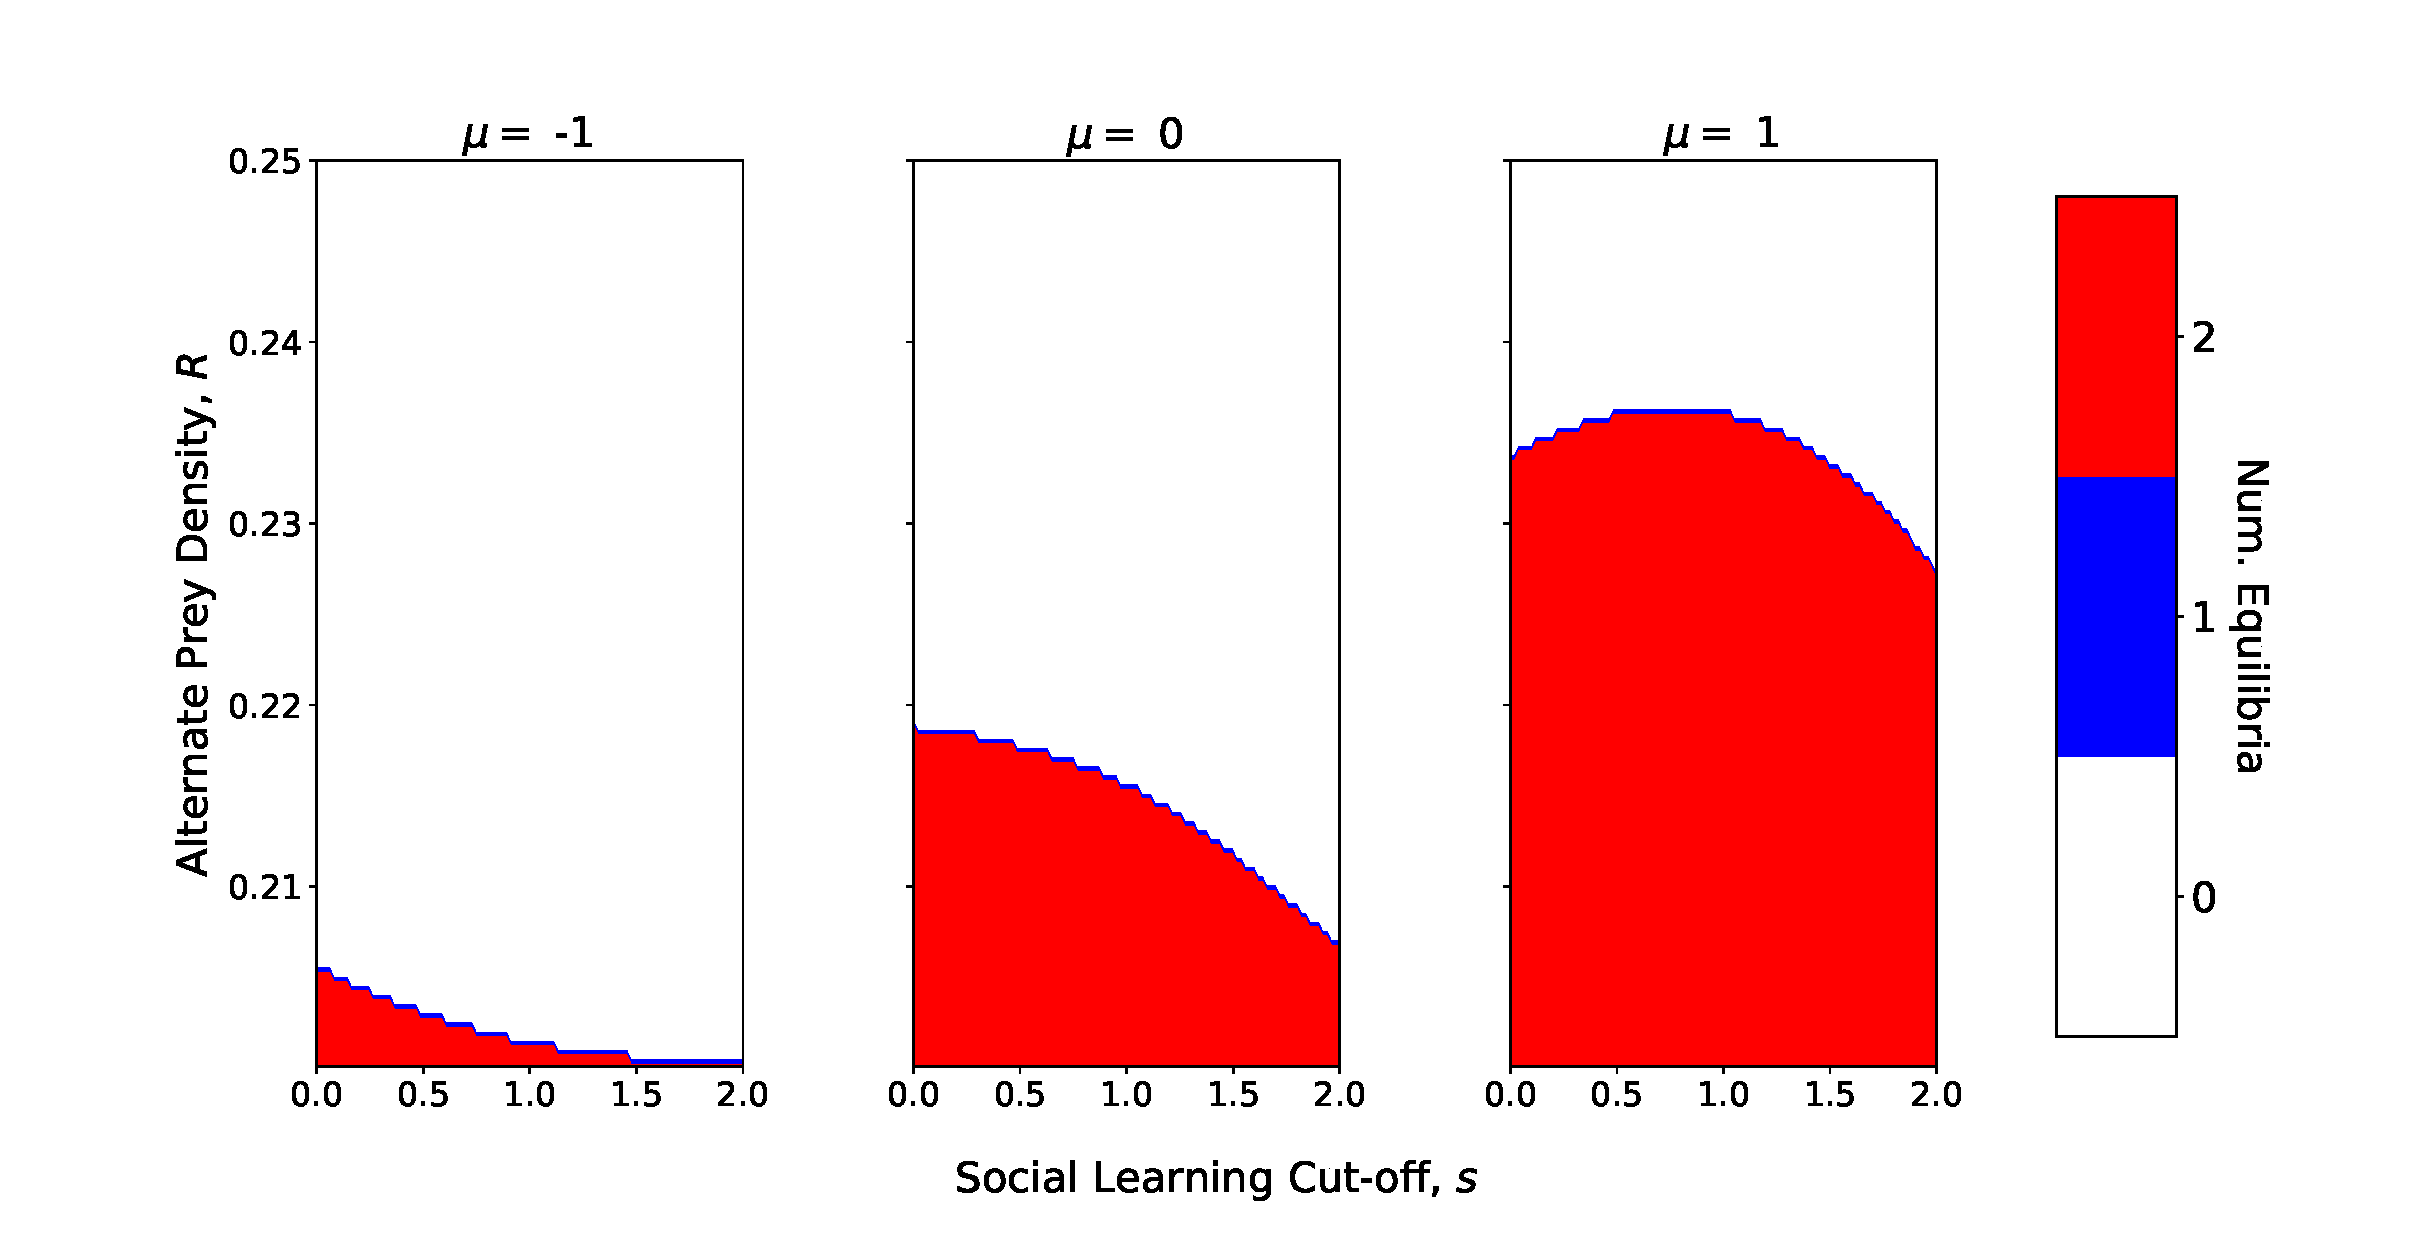
\includegraphics[width= 0.9\textwidth]{Figures_NoDelay/NumEquilibria_Rversuss_delta02_close.eps}
\caption{The number of nonzero $\hr$ equilibria for $\delta = 0.2$ and $R > \delta$, where the number of equilibria are indicated by colored regions, in relation to the social learning cut-off $s$ (x-axis) and alternate prey density $R$ for, from left to right, $\mu = -1,0,1$. We show only $R$ values for which $R < 0.25$ because for $R > 0.25$, there are no nonzero $\hr$ equilibria. }
\label{NoDelay_NumEq_close}
\end{center}
\end{figure}

\begin{figure}[htbp]
\begin{center}
\includegraphics[width= 0.9\textwidth]{Figures_NoDelay/Trajectories_R01_delta02_beta005_muNeg05_s1time.jpg}
\caption{Trajectories of the predator population size $N_p$ (blue), relative population density, $r$ of CP (red), and frequency $u_r$ of predators on CP (purple) with respect to time (in generations).  The parameters are: $R = 0.1, \delta = 0.2, \beta = 0.05, \mu = -0.5,$ and $s = 1$.The left y-axis is the number of individuals in the predator population, and the right y-axes are frequencies ($u_r$ or $r$), from 0 to 1. }
\label{NoDelay_traj1_time}
\end{center}
\end{figure}

\begin{figure}[htbp]
\begin{center}
\includegraphics[width= 0.9\textwidth]{Figures_NoDelay/Trajectories_R01_delta02_beta005_muPos05_s0time.jpg}
\caption{Trajectories of the predator population size $N_p$ (blue), relative population density, $r$ of CP (red), and frequency $u_r$ of predators on CP (purple) with respect to time (in generations). The parameters are: $R = 0.1, \delta = 0.2, \beta = 0.05, \mu = 0.5,$ and $s = 0$. The left y-axis is the number of individuals in the predator population, and the right y-axes are frequencies ($u_r$ or $r$), from 0 to 1. }
\label{NoDelay_traj1_time}
\end{center}
\end{figure}


\begin{figure}[htbp]
\begin{center}
\includegraphics[width= 0.9\textwidth]{Figures_NoDelay//Trajectories_R01_delta02_beta01.jpg}
\caption{Trajectories of the predator population size $N_p$, relative population density, $r$ of CP, and frequency $u_r$ of predators on CP, indicated by the y-axis, x-axis, and line colors, respectively, for 500 time steps. Arrows indicate the direction of the trajectory. Nonzero resource equilibria are indicated by stars, which are colored according to their $\hu_r$ values. For all four figures, $R = 0.1$, $\delta = 0.2$, and $\beta = 0.1$. For the top row of figures, the mean information quality is $\mu = -0.5$ and for the bottom row it is $\mu = 0.5$. For the figures on the left, there is no social learning i.e. $s = 0$, and for the figures on the right, the social learning cut-off is $s = 1$. All trajectories either end at the $\hr = \hN_p = 0$ equilibrium or the polymorphic equilibrium in which $\hN_p, \hr > 0$. The equilibria with at least one population going extinct (not marked with a star) are $\hr = \hN_p = 0$ and $\hN_p = 0$, $\hr = 1$. BUT WHAT ARE THE STABILITIES OF THESE LAST TWO CASES. The magnitudes of the $J^*$ eigenvalues of the polymorphic equilibria, as calculated by \eqref{Jstar_evals_nodelay}, are all less than one for each plot, indicating internal stability.}
\label{NoDelay_traj1}
\end{center}
\end{figure}

\begin{figure}[htb]
\centering
 \begin{subfigure}[b]{.4\textwidth}
	\centering
	\caption{$R = 0.1, \delta=0.5$}
	\includegraphics[width=0.95\textwidth]{Figures_NoDelay/Result3_1_R01_D05.jpg}
	\label{fig:result3_1a}
 \end{subfigure}
  \begin{subfigure}[b]{.4\textwidth}
	\centering
	\caption{$R=0.3, \delta=0.5$}
	\includegraphics[width=0.95\textwidth]{Figures_NoDelay/Result3_1_R03_D05.jpg}
	\label{fig:result3_1b}
 \end{subfigure}
 \newline
  \begin{subfigure}[b]{.4\textwidth}
	\centering
	\caption{$R=0.1, \delta=0.2$}
	\includegraphics[width=0.95\textwidth]{Figures_NoDelay/Result3_1_R01_D02.jpg}
	\label{fig:result3_1c}
 \end{subfigure}
   \begin{subfigure}[b]{.4\textwidth}
	\centering
	\caption{$R=0.6, \delta=0.8$}
	\includegraphics[width=0.95\textwidth]{Figures_NoDelay/Result3_1_R06_D08.jpg}
	\label{fig:result3_1d}
 \end{subfigure}
 \caption{}
  \label{fig:result3_1}
\end{figure}


\begin{figure}[htbp]
\begin{center}
\includegraphics[width=0.9\textwidth]{Figures_NoDelay//N_vs_s_R1delta3.jpg}
\caption{Equilibrium population size (vertical axis; $\hN_p$) versus social learning cut-off (horizontal axis; $s$) for $\mu = 0, \beta = 0.05$ (red line), $\mu = -0.5, \beta = 0.05$ (blue line), $\mu = 0, \beta = 0.02$ (red dots), $\mu = -0.5, \beta = 0.2$ (blue dots).}
\label{N_vs_s_R1delta3}
\end{center}
\end{figure}

\begin{figure}[htbp]
\begin{center}
\includegraphics[width=0.9\textwidth]{Figures_NoDelay//N_vs_s_R2delta3.jpg}
\caption{Like Fig. \ref{N_vs_s_R1delta3}, but $R - 0.2$ and $\delta = 0.3$. \red{Will fill in caption}}
\label{N_vs_s_R2delta3}
\end{center}
\end{figure}

\break

\begin{figure}[htbp]
\begin{center}
\includegraphics[width=0.9\textwidth]{Figures_NoDelay//Optimals_RlessthanDelta.jpg}
\caption{The value of $s$, called $s*$ (vertical axis), which maximizes the predator population size at equilibrium, $\hN_p$, relative to mean environmental information quality $\mu$ (horizontal axis).}
\label{optimal_s_nodelay_RlessthanD}
\end{center}
\end{figure}

\begin{figure}[htbp]
\begin{center}
\includegraphics[width=0.9\textwidth]{Figures_NoDelay//Optimals_RlessthanDelta_muNeg025.jpg}
\caption{The value of $s$, called $s*$ (vertical axis), which maximizes the predator population size at equilibrium, $\hN_p$ relative to the frequency of AP, $R$ (horizontal axis) for mean environmental information quality $\mu = -0.25$.}
\label{optimal_s_nodelay_RlessthanD_R}
\end{center}
\end{figure}
%
%\begin{figure}[htbp]
%\begin{center}
%\includegraphics[width= 0.9\textwidth]{Figures_NoDelay//Trajectories_R01_delta02_beta005.jpg}
%\caption{Trajectories of the predator population size $N_p$, relative population density,$r$ of CP, and frequency $u_r$ of predators on CP, indicated by the y-axis, x-axis, and line colors, respectively, for 500 time steps. For all four figures, $R = 0.1$, $\delta = 0.2$, and $\beta = 0.05$. For the top row of figures, the mean information quality is $\mu = -0.5$ and for the bottom row it is $\mu = 0.5$. For the figures on the left, there is no social learning i.e. $s = 0$, and for the figures on the right, the social learning cut=off is $s = 1$. Nonzero resource equilibria are indicated by stars, which are colored according to their $\hu_r$ values. }
%\label{NoDelay_traj2}
%\end{center}
%\end{figure}
%
%\begin{figure}[htbp]
%\begin{center}
%\includegraphics[width= 0.9\textwidth]{Figures_NoDelay//Trajectories_R01_delta02_beta0025.jpg}
%\caption{Trajectories of the predator population size $N_p$, relative population density,$r$ of CP, and frequency $u_r$ of predators on CP, indicated by the y-axis, x-axis, and line colors, respectively, for 500 time steps. For all four figures, $R = 0.1$, $\delta = 0.2$, and $\beta = 0.025$. For the top row of figures, the mean information quality is $\mu = -0.5$ and for the bottom row it is $\mu = 0.5$. For the figures on the left, there is no social learning i.e. $s = 0$, and for the figures on the right, the social learning cut-off is $s = 1$. Nonzero resource equilibria are indicated by stars, which are colored according to their $\hu_r$ values. }
%\label{NoDelay_traj2}
%\end{center}
%\end{figure}
%
%\begin{figure}[htbp]
%\begin{center}
%\includegraphics[width= 0.9\textwidth]{Figures_NoDelay//Trajectories_R021_delta02_beta0025.jpg}
%\caption{Trajectories of the predator population size $N_p$, relative population density,$r$ of CP, and frequency $u_r$ of predators on CP, indicated by the y-axis, x-axis, and line colors, respectively, for 500 time steps. For all four figures, $R = 0.21$, $\delta = 0.2$, and $\beta = 0.025$. For the top row of figures, the mean information quality is $\mu = -0.5$ and for the bottom row it is $\mu = 0.5$. For the figures on the left, there is no social learning i.e. $s = 0$, and for the figures on the right, the social learning cut-off is $s = 1$. Nonzero resource equilibria are indicated by stars, which are colored according to their $\hu_r$ values. On the top row, the resource equilibria are $\hat{r} = .122, .056$ on the left and there are no equilibria on the right.  On the bottom row, the resource equilibria are $\hr = .179, .017$ on the left and $\hr = .183,.018$ on the right. Each trajectory in the top right plot has $N \to \infty$, and $r \to 0$. }
%\label{NoDelay_traj3}
%\end{center}
%\end{figure}
%
%
%
%\begin{figure}[htbp]
%\begin{center}
%\includegraphics[width= 0.9\textwidth]{Figures_NoDelay//Trajectories_R04_delta02_beta0025t10.jpg}
%\caption{Trajectories of the predator population size $N_p$, relative population density,$r$ of CP, and frequency $u_r$ of predators on CP, indicated by the y-axis, x-axis, and line colors, respectively, for 10 time steps. For all four figures, $R = 0.4$, $\delta = 0.2$, and $\beta = 0.025$. For the top row of figures, the mean information quality is $\mu = -0.5$ and for the bottom row it is $\mu = 0.5$. For the figures on the left, there is no social learning i.e. $s = 0$, and for the figures on the right, the social learning cut-off is $s = 1$. There are no nonzero resource equilibria, and instead $r \to 0$ and $N \to \infty$ (not shown). }
%\label{NoDelay_traj4}
%\end{center}
%\end{figure}

%and \eqref{freqs_allB}a - \eqref{freqs_allB}b at equilibrium are
%\begin{subequations}
%\begin{align}
%(1 + \delta) u_r &= L_u(u_r,r)(1+r) \\
%(1 + \delta)(1-u_r) &= L_u(u_r)(1+R).
%\end{align}
%\end{subequations}
%
%\subsubsection{Equilibria, no time delay}
%The resource population dynamics are
%\begin{equation}
%r' = \frac{r(2 - \beta N_p L_u(u_r,r))}{1 + \eta r} 
%\end{equation}
%because all predators are $B$, but at equilibrium 
%\begin{equation}
%r = 1 - \beta \hN_p L_u(\hu_r, r).
%\end{equation}
%
%IF DELTA IS R...
%
%OTHERWISE...
%
%Substituting \eqref{delta_eq} for $\L_u(\hu_r, \hr)$, the equilibrium $\hN_p$ is
%
%which can also be rearranged into the equation $Q^{(1)}_r(r) = 0$ where
%\begin{equation} \label{Q_1_r}
%Q^{(1)}_r(r) = r^2 -r(1+R) + R + \beta \hN_p(\delta-R).
%\end{equation}
%The $r^*$ that minimizes $Q^{(2)}_r(r)$ is $r^* = \frac{1+R}{2},$ at which 
%$$
%Q^{(2)}_r(r^*) = -\frac{1}{4}(1 - R)^2 + \beta \hN_p(\delta - R),
%$$ 
%and thus $Q^{(2)}_r(r)$ has two roots if 
%$$
%\hN_p < \frac{(1-R)^2}{4\beta(\delta - R)}.
%$$
%which also means that for $\hr>0$ to exist, $\delta > R$. If $\delta < R$, then the forager population can grow infinitely even if the CP is depleted, so it will deplete the CP.
%
%Furthermore, the equation
%\begin{equation} \label{hr_notsolved}
%r = 1 - \beta N_p (K u_r + \frac{r}{r+R} \pc)
%\end{equation}
%can be rearranged into the quadratic equation $Q^{(2)}_r(r) = 0$ where 
%\begin{equation}\label{Q_r_nodelay_2}
%Q_r^{(2)}(r) = r^2 + r\lrb{R - 1 + \beta N_p (K\hu_r + \pc)} + R \lrp{-1 + \beta \hat{N}_p K \hu_r }.
%\end{equation}
%
%Since $Q_r^{(1)}(r) = Q_r^{(2)}(r) = 0$,
%\begin{equation}
%\hr = \frac{2R - \beta \hN_p \lrb{R(1+K \hu_r) - \delta}}{2R + \beta \hN_p(K \hu_r + \pc)}.
%\end{equation}
%which exists if
%
%
%
%%%
%
%CHECK NUMERICALLY
%
%
%% OLD STUFF:
%
% If every individual in the population carries allele $B$, then if $N_p < 1/\beta$, we can to find the nonzero CP density equilibrium in one of two ways. The first way substitutes $L_{tot} = K \hu_r + \pc \frac{r}{r+R}$ into \eqref{r_hat_nodelay}, and the second way substitutes \eqref{delta_eq} for $L_{tot}$ in \eqref{r_hat_nodelay}. Starting with the first method,
%
%As for the second method of solving for the nonzero CP density equiibrium,
%\begin{equation}
%\hr = 1 - \beta \hN_p \lrp{ \frac{\delta-R}{r-R}}
%\end{equation}
%which can be rearranged into the equation $Q^{(2)}_r(r) = 0$ where
%\begin{equation}
%Q^{(2)}_r(r) = r^2 -r(1+R) + R + \beta \hN_p(\delta-R)
%\end{equation}
%where the $r^*$ that minimizes $Q^{(2)}_r(r)$ is $r^* = \frac{1+R}{2},$ at which 
%$$
%Q^{(2)}_r(r^*) = -\frac{1}{4}(1 - R)^2 + \beta \hN_p(\delta - R),
%$$ 
%and thus $Q^{(2)}_r(r)$ has two roots if 
%$$
%\hN_p < \frac{(1-R)^2}{4\beta(\delta - R)}.
%$$
%which also means that for $\hr>0$ to exist, $\delta > R$. If $\delta < R$, then the forager population can grow infinitely even if the CP is depleted, so it will deplete the CP.
%
%
%
%The equilibrium population size $\hN_p$ can be found in terms of $\hu_r$ and $\hr$ by substituting \eqref{r_hat_nodelay} into \eqref{W_allB}. Then
%$$
%R + L_u(\hu_r, \hr) (1 - \beta N_p L_u(\hu_r,\hr) - R)  - \delta = 0 
%$$
%and hence if $L_u(\hu_r,\hr) > 0$
%\begin{equation}\label{hN_p_solved}
%\hN_p = \frac{1}{\beta \lrp{L_u(\hu_r,\hr)}^2} \lrb{R - \delta + L_u(\hu_r,\hr) (1 - R) }
%\end{equation}
%and if $L_u(\hu_r, \hr) = 0$ the population grows infinitely.

%\red{I just tried simulations in which $R > \delta$ and $R < \delta$. For both, $\delta = 0.2$, $K = 0.3$, $\pc = 0.4$, and initially $u_r = 0$, $u_R = 1$, $x = 0$, $r = 0.8$, $N = 100$, and $\beta = 0.01$. 
%\begin{enumerate}
%\item For $R = 0.5$, the population size $N_p$ grew infinitely and $r \to 0$ (didn't do enough rounds to determine if $\hr = 0$.)
%\item For $R = 0.1$, the system went to the equilibrium $\hw = 1.2 = 1 + \delta$,  $\hu_r = 0.5002$, $\hu_R = 0.4998$,  $\hN_p = 149.5423$, and $\hr = 0.3199$ (rounded to the fourth decimal place). Equations (18) and (20) fit with these results the value of $\hr$ did not match any of the roots of $Q_r^{(1)}(r)$ nor $Q_r^{(2)}(r)$. I'm having trouble figuring out where I made a mistake.
%\end{enumerate}
%}

%
%
%The equilibrium population size of predators, $\hN_p$, and the equilibrium frequency of predators foraging for the CP, $\hu_r$, are solved by substituting the nonzero value of $\hr$. %, \red{which is the larger root of $Q_r(r)$ in \eqref{Q_r_nodelay}, into Eqs. \eqref{hN_p_solved_nice}and \eqref{freqs_allB}a - b?}.
%
%The equilibrium frequency at which predators feed on prey can be found in terms of $\hr$. From \eqref{sys_allB}c,
%\begin{equation}
%(1 + \delta) u_r = \frac{(\delta-R)}{\hr-R}(1 + \hr)
%\end{equation}
%and from \eqref{sys_allB}c,
%\begin{equation}
%(1 + \delta) (1 - u_r) = \frac{(\hr - \delta)}{\hr-R}(1+R)
%\end{equation}
%\subsection{Equilibria, time delay}
%Here, $\hr = 1 - \beta \hu_r \hN$. From \eqref{sys_allB}c-d, at equilibrium
%\begin{equation}
%\frac{u_r}{1 - u_r} = \frac{L(u_r,r)(1+r)}{(1 - L(u_r,r))(1+R)}
%\end{equation}
%
%, which can be positive or negative, $Q_r(\alpha-1) = N_p\beta \lrb{ K \alpha u_r + \pc(\alpha - 1)}> 0$ and also $Q_r(\alpha-1) > Q_r(0)$ because $\alpha > 1$. 
%TO DETERMINE THE NUMBER OF EQUILIBRIA IN_p QR(0) IS POSITIVE, WE NEED TO EXAMINE WHERE THE MINIMUM IS. IF IT'S POSITIVE, NO ROOTS. IF NEGATIVE, TWO ROOTS. MAY WANT TO ALSO LOOK AT THE DERIVATIVE OF Q AT 0 The vertex of $Q_r(r)$ is at
%$$
%r^* = \frac{1}{2} \lrb{\alpha - 1 - A - \beta \hat{N_p}(K\hu_r + \pc)} > 0, %should this be - 
%$$
%and thus the minimum value of $Q_r(r)$ is
%\begin{equation}
%Q(r^*) = - r^*2 + \beta \hN_p K \hu_r - A(\alpha-1). FIX THIS
%\end{equation}
%\red{
%Since $Q(\alpha - 1) > Q(0)$, the vertex $r^* < \alpha - 1$.
%We have the following conditions which determine how many nonzero prey population size equilibria exist if $\beta > 0$:
%\begin{enumerate}
%\item If $Q(r^*) > 0$ then there is no prey population size equilibrium. Note that if $Q(r^*) > 0$ then also $Q(0) > 0$.
%\item If $Q(r^*) < 0$ and $Q_r(0) > 0$ then there are two equilibrium prey population sizes.
%\item If $Q(r^*) < 0$ and $Q_r(0) < 0$ then there is one equilibrium prey population size and it is the larger of the two roots of $Q_r(r)$.
%\end{enumerate}}


%
%\section{Continuous Version
% A population of predators of density $y(t)$ at time $t$ hunts for two types of prey with respective densities denoted $x_i(t)$ at time $t$ for $i = 1,2$. Only predators who have successfully learned how to find food can reproduce. The two prey types have density-dependent growth due to intra-type competition but do not compete with each other, i.e. there is no inter-type competition. Let $\vec{x}(t) = [x_1,x_2]^T$. The intrinsic rate of growth for prey population $i$ is $R_i$ and the carrying capacity is $K_i$ for $i = 1,2$.
% 
% Let $\psi_i(t)$ be the probability at time $t$ that a predator has learned the appropriate behavior to catch prey $i$, defined below in Section \ref{secLearning}. Also write $\vec{\psi} = [\psi_1,\psi_2]^T$. The probability of catching a prey type and the amount of that food type that is available together determine a predator's functional response, or kill rate, $f_i (t)$, which is defined below in Section \ref{funcresponse}. The conversion rate of prey to predator density growth per unit time is $a_i$ for $i = 1,2$ and the death rate of predators is $\delta$. The effect of predation on the prey population per unit time is $\gamma_i$. Thus system dynamics are described by 
%\begin{subequations}
%\begin{align}
%\frac{dy}{dt} =& y \lrp{ a_1  f_1(t)+ a_2 f_2(t)- \delta } \\
%\frac{dx_i}{dt} =& R_i x_i(t) \lrp{ 1 - \frac{x_i(t) }{K_i} } - \gamma_i y(t) f_i\lrp{\vec{x}(t), \vec{\psi}(t) },
%\end{align}
%\end{subequations}
%as illustrated by the following diagram.
%\vspace{1cm}
%
%\tikzstyle{predators} = [rectangle, draw, fill = blue!20, minimum width =4cm, minimum height = 7 cm, node distance= 10cm, text depth=6cm]
%\tikzstyle{committed} = [rectangle, draw, fill = green!20, minimum width = 3.5cm, minimum height = 2cm, text width = 3 cm]
%\tikzstyle{food} = [ellipse, draw, fill = yellow!20,
%	text width = 4.5em, text centered, node distance= 5cm]
%\tikzstyle{line} = [draw, very thick, color=black, -{Latex}]
%\tikzstyle{inhibit} = [draw, very thick, color=black, -{Square}]
%\begin{tikzpicture}
%	% Place nodes
%	\draw (0,0) node[predators] (predators) {All Predators};
%	\draw(0,1.5) node[committed] (committed_1) {Predators feeding on resource $1$};
%	\draw(0,-1.5) node[committed] (committed_2) {Predators feeding on resource $2$};
%	\draw (7,1.5) node [food] (food_1) {N_pood type $1$};
%	\draw (7,-1.5) node [food] (food_2) {N_pood type $2$};
%	% Place edGes	
%	\path [inhibit] (committed_1) -- node {} (food_1);
%	\path [inhibit] (committed_2) -- node {} (food_2);
%	\path [line] (committed_1) to [out=170,in=175, looseness = 5]  node{} (predators);
%	\path [line] (committed_2) to [out=190,,in=185, looseness = 5]  node{} (predators);
%	% Label edGes
%	\draw (-3,2.5) node (birth1) {Birth};
%	\draw (-3,-2.5) node (birth2) {Birth};
%	\draw (3.5,2) node (pred1) {Predation};
%	\draw (3.5,-2) node (pred2) {Predation};
%\end{tikzpicture}
%%
%\subsection{N_punctional Response} \label{funcresponse}
%
%The simplest version of the functional response is a Type I response where the kill rate is linearly related to the amount of prey available \cite{holling1959some}. A variation of the Type I response which takes into account the effect of learning is 
%\begin{equation} \label{funcresponse_lin}
%f_i \lrp{\vec{x}(t), \vec{\psi}(t)}= f_i \lrp{x_i(t), \psi_i(t)} = \psi_i(t) x_i(t).
%\end{equation}
%% Check this ^
%
%A more realistic but less tractableversion is the Type II response \cite{holling1959some}, which can be adjusted to include the effect of learning using the functional response from \cite{van2001alternative},
%\begin{equation} \label{funcresponse_ii}
%f_i\lrp{\vec{x}(t), \vec{\psi}(t)} = \frac{ \psi_i(t)x_i(t) }{ 1 + \sum_{i=1,2} \psi_i(t) T_i x_i(t) },
%\end{equation}
%where $T_i$ is the handling time for prey $i$.
%
%\subsection{Learning} \label{secLearning}
%Predators can learn socially with probability $L_s$ or individually with probability $L_I$ where $L_s + L_I = 1$.  Individual learning occurs when a predator adopts an appropriate hunting behavior through directly sampling the environment.  Predators that learn through trial-and-error should become better at catching prey if they encounter them more frequently. Assume the rate at which a predator encounters prey is proportional to the density of the prey population. When predators individually learn to catch prey, the killed prey acts as a reinforcement to the behavior, and thus this behavior can be thought of as a conditioned response. Researchers studying conditioned learning use a learning curve that is the plot of how the performance of a conditioned behavior changes in relation to the number of trials that resulted in reinforcement \cite{gallistel2004learning}. Group learning curves, which average the learning curves over a set of individuals, often are approximated using the Weibull function \cite{gallistel2004learning}. While individuals learning curves often have steps rather than a gradual increase \cite{gallistel2004learning}, we assume a group-learning curve since the predator-prey model involves learning over a population rather than at the individual level. Let $\sigma_i(x_i)$ be the probability of individually learning a successful hunting strategy for prey $i$ as a function of the amount of prey $i$ available, which is a proxy of the number of reinforcements the predator experiences.  Therefore
% \begin{equation} \label{indlearn}
% \sigma_i(x_i) = 1 - \exp\lrp{-\lrp{\frac{x_i}{b_i}}^{c_i} },
% \end{equation}
%  where $b_i>0$ is the latency of behavioral onset and $c_i>0$ is the abruptness, or steepness, at which the behavioral performance increases \cite{gallistel2004learning}. Since $x_i \geq 0$, $0 \leq \sigma_i(x_i) \leq 1$.  In this case,
% \begin{equation}
% \sigma_i'( x_i) = c_i b_i^{-c_i} x^{c_i-1} \exp\lrp{ -(x_i/b_i)^{c_i}}
% \end{equation}
% and
% \begin{equation}
% \sigma_i''( x_i)  = \sigma_i'(x_i) x_i^{-1} \lrp{ c_i - 1 -c_ib_i^{-c_i} x^{c_i}}.
% \end{equation}
%The inflection point is at
%\begin{align}
%x_i^* = b_i \lrp{ 1-\frac{ 1}{c_i}}^{1/c_i}
%\end{align}
%if $0 < c_i \leq 1$ so that $x_i^* > 0$. Otherwise the learning curve does not have an inflection point and resembles a reverse exponential. Since $x_i \leq K_i$, if we want the learning curve to have an inflection point over the domain $0 \leq x_i \leq K_i$, then $b_i \lrp{ 1-\frac{ 1}{c_i}}^{1/c_i} \leq K_i$. 
%
%\begin{figure}[htbp!]
%\centering
%\begin{tikzpicture}
%\begin{axis}[mystyle, xmin=0, ymin=0]
%	\addplot[domain=0:5, samples=100, color=red]{1-exp(-(x)^2)};
%	\addplot[domain=0:5, samples=100, color=blue]{1-exp(-(x/3)^2)};
%	\addplot[domain=0:5, samples=100]{1-exp(-(x)^1)};
%	%\addplot[domain=0:5, samples=100]{1-exp(-(x/2)^1)};
%	%\addplot[domain=0:5, samples=100]{1-exp(-(x)^3)};
%\end{axis}
%\end{tikzpicture}
%\caption{Plots of $\sigma_i(x_i)$ as in Eq. \eqref{indlearn} with $b_i = 1, c_i = 2$ (red) $b_i=3,c_i=2$ (blue), and $b_i=1, c_i=1$ (black).}
%\end{figure}
%
%% However, if we assume that individuals at time $t$  know only one out of two behaviors, which would require that $\sigma_1(x_1) + \sigma_2(x_2) \leq 1$, then we can set
%%  \begin{equation} \label{indlearn2}
%%  \sigma_i(x_i) =
%% \begin{cases}
%% \frac{x_i}{x_1 + x_2} \lrp{ 1 - \exp \lrp{-\lrp{\frac{x_i}{b_i}}^{c_i} }}  & \text{if } x_1 + x_2 > 0 \\
%% 0 & \text{otherwise}
%% \end{cases}
%%  \end{equation}
%
%%where the term $\frac{x_i}{x_1 + x_2}$ ensures that $\sigma_1(x_1) + \sigma_2(x_2) \leq 1$ if $x_1 + x_2 > 0$. 
% 
%Social learning occurs when a na\"{i}ve predator imitates a more experienced predator hunting prey. Let $\tau$ be the time delay indicating that the demonstrator is from an earlier generation. The structure of the model depends on assumptions about social learning. There are three options
%
%\begin{enumerate}
%% Unbiased social learning
%
%\item[SL1:] Assume the probability that a predator using social learning adopts behavior $i$ is
%\begin{equation}\label{soclearn_unbiased}
%S\lrp{\psi_i(t-\tau)} = \psi_i(t - \tau).
%\end{equation}
%In this case we do not have to assume that a predator only knows how to perform one behavior at a time, so if individual learning is defined in Eq. \eqref{indlearn}, then
%\begin{equation}
%\psi_i(t) = L_s \psi_i(t-\tau) + L_I \sigma_i(x_i(t)).
%\end{equation}
%If the equilibrium $(\hx_1,\hx_2,\hy)$ exists, (see below for discussion of conditions for existence), then since $L_s = 1 - L_I$, $\hp_i = \sigma_i(\hx_i)$ if $L_I > 0$  and otherwise if $L_I=0,L_s=1$ then $\psi_i(t) = \psi_i^{(0)}$. Therefore if $L_I > 0$ the system dynamics do not depend on the probability that individuals use social learning and is thus not very interesting and contradicts the results of \cite{borofsky2020conformity}.  IT'S REALLY STRANGE I GET THIS RESULT, BUT IN \cite{borofsky2020conformity} \red{THE EQUILIBRIA For K=D=0 AND K>0 D=0 WERE DIN_pN_pERENT. WHY? IS IT BECAUSE IN \cite{borofsky2020conformity} THE RECURSION For $u_i$ HAS A N_pITNESS? SHOULD MY EQUATION For $\psi_i$ HAVE N_pITNESS?}
%% Biased social learning
%\item[SL2:] If social learners only imitate predators performing successful hunting strategies then Eqn \eqref{soclearn_unbiased} becomes
%\begin{equation} \label{soclearn_biased1}
%S_i \lrp{t} = 
%\begin{cases}
%\frac{\psi_i(t-\tau)}{\psi_1(t-\tau) + \psi_2(t-\tau)} & \text{if } \psi_1(t-\tau) + \psi_2(t-\tau) > 0\\
%0 & \psi_1(t-\tau) + \psi_2(t-\tau) = 0
%\end{cases}
%\end{equation}
%where we must also assume that time $t$ a predator either performs behavior 1 and 2, so $\psi_1 + \psi_2 \leq 1$ and $1 - \psi_1 - \psi_2$ is the probability a forager performs an unsuccessful foraging behavior. Then individual learning is defined by Eq. \eqref{indlearn} scaled by $\frac{x_i}{x_1+x_2}$and
%\begin{subequations} \label{eqPsi_biased}
%\begin{align}
%\psi_i(t) &=L_I  \frac{x_i}{x_1+x_2} \sigma_i(x_i(t)) + L_s S_i(t).
%\end{align}
%\end{subequations}
%If predators only use individual learning, i.e. $L_I = 1$ and $L_s = 0$, then at equilibrium $\hp_i = \frac{\hx_i}{\hx_1 + \hx_2} \sigma_i(\hx_i)$. If predators only use social learning, i.e. $L_s = 1$ and $L_I = 0$, then $(\hp_i,\hp_j) = (0,0)$ or $(p, 1-p)$ for some constant $p$ such that $0 \leq p \leq 1$ and $i,j = 1,2$, $i \neq j$. Otherwise if $L_I,L_s>0$ then we solve the pair of equations obtained by substituting \eqref{soclearn_biased1} into \eqref{eqPsi_biased}. Using the Python package Sympy, I found that the equilibria are $(\hp_1, \hp_2) = (0,0)$ and
%\begin{equation} \label{socAssumption2}
% (\hp_1,\hp_2) = \lrp{ \frac{L_I }{\hx_1+\hx_2}+ \frac{L_s }{\hx_1 \sigma_1(\hx_1)+\hx_2 \sigma_2(\hx_2)} }(\hx_1 \sigma_1(\hx_1),\hx_2 \sigma_2(\hx_2)).
%\end{equation}
%where the latter equilibrium only exists if $\hx_1 + \hx_2 > 0$ and $\hx_1 \sigma_1(\hx_1) + \hx_2 \sigma_2(\hx_2) > 0$. 
%
%
%If we look at social learning where social learners copy members of the same generation, then we substitute $\tau = 0$ into Eq. \eqref{eqPsi_biased}, i.e. $S_i(t) = \frac{\psi_i(t)}{\psi_1(t) + \psi_2(t)}$. Solving for $\psi_i(t)$ yields
%\begin{equation} \label{eqPsi_SL2_nodelay}
%\psi_i = \psi_i(x_1, x_2) = x_i \sigma_i(x_i) \lrp{\frac{L_I}{x_1+x_2} + \frac{L_s}{x_1 \sigma_1(x_1)+x_2 \sigma_2(x_2)}}.
%\end{equation}
%The above equation is illustrated in N_pigure \ref{fig:psi_no_delay}. 
%\begin{figure}[htbp]
%\begin{center}
%\includegraphics[width=0.95\textwidth]{psi_no_delay.png}
%\caption{Graphs of Equation \eqref{eqPsi_SL2_nodelay} for $b_1=b_2=1$, $c_1 = c_2=2$ where $x_1 \in [0.01,1]$. For each graph, the horizontal axis is $x_1$ and the vertical axis is $\psi_1(x_1)$. The value of $x_2$ is held constant for each graph. On the top row, it is constant at $x_2 = 0$ on the left and $x_2 = 0.2$ on the right. On the bottom row, it is held constant at $x_2 = 0.5$ on the left and $x_2 = 0.9$ on the right.  Lines are colored by the $L_I$ value, using the same color to $L_I$ value correspondence for each graph. where the corresponding social learning value is $L_s = 1 - L_I$}.
%\label{fig:psi_no_delay}
%\end{center}
%\end{figure}
%
%
%
%% N_pILL IN!
%
%% SL3: Social learners imitate actions not individuals
%\item[SL3:] If we want social learners to only learn from successful behavior but also allow $\psi_i \leq 1$ without requiring $\psi_1 + \psi_2 \leq 1$, then we can have social learners imitate successful hunting events rather than individuals, i.e. the probability of socially learning behavior $i$ is proportion to the functional response or kill rate of prey $i$, $f_i(t-\tau)$. Thus
%%
%\begin{equation} \label{soclearnactions}
%S_i(t) = W_i f_i(t-\tau)
%\end{equation}
%%
%where $W_i$ ensures that $S_i(t) \leq 1$. For example, $W_i$ can be the inverse of the maximum or upper bound of the functional response as $x_i$ becomes large, depending on how $f_i(t)$ is defined (see Section \ref{funcresponse}). If the functional response is linear as in Eq. \eqref{funcresponse_lin}, then we can set $W_i = \frac{1}{K_i}$ since $X_i \leq K_i$ and $\psi_i \leq 1$.  Individual learning can be defined as in \eqref{indlearn} and 
%\begin{equation}
%\psi_i(t) = L_I \sigma_i(x_i) + L_s W_i \psi_i(t-\tau)x_i
%\end{equation}
%so
%\begin{equation}
%\hp_i = \frac{L_I \sigma_i(\hx_i)}{1-L_s W_i \hx_{i}}.
%\end{equation}
%
%N_purthermore, if $\tau = 0$ then 
%\begin{equation}
%\psi_i = \frac{L_i \sigma(x_i)}{1-L_s W_i x_i}.
%\end{equation}
%
%
% If the functional response is Type II as in Eq. \eqref{funcresponse_ii}, then we can set $W_i = T_i$, but since $x_i(t)$ is a density we may get away with having $W_i = 1$. Now the equilibrium value $\hp_i$ might not be possible to find because Python timed out when I tried to find the solution.
% 
% Note that it may make more mechanistic sense to define social learning as
%\begin{equation}
%S_i(t) = \frac{ f_i(t-\tau)}{f_1(t-\tau) + f_2(t-\tau)}
%\end{equation}
%but Eq \eqref{soclearnactions} is easier to analyze. 
%\end{enumerate}
%
%
%
%\subsection{Simplifying assumptions}
%Assume that all dynamics are equivalent for both prey populations, i.e. $R_1 = R_2 = R$, $K_1 = K_2 = K$, $T_1 = T_2 = T$, $a_1 = a_2 = a$, $\gamma_1 = \gamma_2$, $b_1 = b_2 = b$, and $c_1 = c_2 = c$.
%%Assume that the parameters for the intrinsic growth rate and carrying capacity of each prey species is the same, so $R_1 = R_2 = R$ and $K_1 = K_2 = K$, N_purther assume, that catching prey from either species requires the same handling time, i.e. $T_1 = T_2 = T$, conversion to predator biomass, i.e. $a_1 = a_2 = a$, and that the independent learning curves are the same, i.e. $b_1 = b_2 = b$ and $c_1 = c_2 = c$. 
%Then for some positive real number $x$, let $\sigma(x)  = \sigma_1(x)= \sigma_2(x)$. Also let $S(t) = S_1(t) = S_2(t)$.
%
%
%If we use a linear functional response, i.e. $f_i(t) = \psi_i(t) x_i(t)$, then we can use dimensional analysis to reparameterize the system. Let $X_i = x_i/K$ and let $Y = Ry/(aK)$. Let $\eta = aK$. Then
%
%\begin{subequations}
%\begin{align}
%\frac{aK}{R} \frac{dY}{dt}&= \frac{aK}{R} y \lrp{aK\psi_1(t) X_1 + aK \psi_2(t) X_2(t) - \delta} \\
%K \frac{dX_i}{dt} &= RKX_i (1 - X_i ) - \gamma \psi_i \frac{aK}{R} KX_i Y_i
%\end{align}
%\end{subequations}
%
%which simplifies to 
%\begin{subequations}\label{sys_lin_newparams}
%\begin{align}
%\dv{Y}{t} &= Y(\eta \psi_1 X_1+ \eta \psi_2 X_2- \delta )\\
%\dv{X_i}{t} &= RX_i(1 - X_i) - A  \psi_i X_i Y.
%\end{align}
%\end{subequations}
%where $A = \frac{\gamma \eta}{R}$. 
%\subsubsection{SL2}
%For assumption SL2,
%\begin{equation}
%\psi_i(t) = L_I \frac{X_i}{X_1+X_2}\sigma(KX_i) + L_s \frac{\psi_i(t-\tau)}{\psi_1(t-\tau) + \psi_2(t-\tau)}
%\end{equation}
%where the equation for $\sigma(KX_i)$ is the same as $\sigma(x_i)$ but with $b$ replaced by $B = K/b$, i.e. 
%\begin{equation}
%\sigma(KX_i) = 1 - \exp\lrp{ \lrp{-BX_i}^c }.
%\end{equation}
%Let $\ts_i = \ts(X_i) = \sigma(KX_i)$. When $\tau = 0$ and $L_I > 0$
%\begin{equation} \label{sl2_no_delay}
%\psi_i(t) = X_i \ts_i \lrp{\frac{L_I}{X_1+X_2} + \frac{L_s}{X_1 \ts_1 + X_2 \ts_2}}.
%\end{equation}
%If $\tau=L_I = 0, L_s = 1$, we have no way to solve for $\psi_i(t)$. 
%
%The partial derivatives of $\psi_i(t)$ from \eqref{sl2_no_delay} with respect to $X_i$ and $X_j$ are
%\begin{multline}
%\pdv{\psi_i}{X_i} = \dv{\ts_i}{X_i} \lrp{  \frac{-L_s X_i^2 \ts_i}{(X_1 \ts_1 + X_2 \ts_2)^2} + \psi_i/\ts_i }  \\- X_i \ts_i \lrp{ \frac{L_I}{(X_1 + X_2)^2 }+ \frac{L_s \ts_i}{(X_1 \ts_1 + X_2 \ts_2)^2}} + \psi_i/X_i
%\end{multline}
%
%and
%\begin{multline}
%\pdv{\psi_i}{X_j}  =  -\dv{\ts_j}{X_j} \frac{L_s X_1 X_2 \ts_i}{(X_1 \ts_1 + X_2 \ts_2)^2}  - X_i \ts_i \lrp{ \frac{L_I}{(X_1 + X_2)^2} + \frac{L_s \ts_j}{(X_1 \ts_1 + X_2 \ts_2)^2} }
%\end{multline}
%for $i \neq j$, where $\dv{\ts_i}{X_i} = cB^c X_i^{c-1} \exp\lrp{ -(BX_i)^c}$.
%
%\subsubsection{SL3}
%For assumption SL3, 
%\begin{equation}
%\psi_i(t) = L_I \ts(X_i) + L_s S_i(t)
%\end{equation}
%where
%\begin{equation}
%S_i(t) = \tilde{W} \psi_i(t - \tau) X_i(t - \tau)
%\end{equation}
%for $\tilde{W} = KW$. When $\tau = 0$, 
%\begin{equation}
%\psi_i(t) = \frac{L_I \ts(X_i)}{1-L_s \tW X_i}.
%\end{equation}
%The partial derivatives with respect to $X_i$ and $X_j$ are
%\begin{equation}
%\pdv{\psi_i}{X_i} = \dv{\ts}{X_i} \frac{L_I}{1-L_s \tW X_i} + \frac{L_s L_I \tW \ts_i}{(1-L_s \tW X_i)^2}
%\end{equation}
%and
%\begin{equation}
%\pdv{\psi_i}{X_j} = 0.
%\end{equation}
%%%%%%%		Analysis		%%%%%%%%
%
%\section{Analysis with no time delay}
%For the subsequent work, assume the functional response is linear as in Eq. \eqref{funcresponse_lin}, i.e. $f_i(t) = \psi_i(t) x_i(t)$ and the predator-prey system is \eqref{sys_lin_newparams}. 
%\subsection{Equilibria and Linear Stability Analysis}
%
%Let $N_p(Y,X_1,X_2) = \frac{dY}{dt}$ and $G_i(Y,X_1,X_2)= \frac{dX_i}{dt}$. The Jacobian is
%\begin{equation} \label{jac}
%J (\hY,\hX_1,\hX_2) = 
%\begin{pmatrix}
%\pdv{N_p}{Y} && \frac{\partial N_p}{\partial X_1} && \frac{\partial N_p}{\partial X_2}\\ \\
%\pdv{G_1}{Y} && \frac{\partial G_1}{\partial X_1} && \frac{\partial G_1}{\partial X_2} \\ \\
%\frac{\partial G_2}{\partial Y} && \frac{\partial G_2}{\partial X_1} && \frac{\partial G_2}{\partial X_2}
%\end{pmatrix}
%\end{equation}
%where at the equilibrium,
%
%\begin{subequations}
%\begin{align}
%\pdv{N_p}{Y} &=\eta \hp_1 \hX_1+ \eta \hp_2 \hX_2- \delta \\
%\pdv{N_p}{X_i} &= \hY \eta \lrp{ \hp_i + \hX_i \pdv{\psi_i}{\hX_i} + X_j \pdv{\psi_j}{\hX_i}} \\
%\pdv{G_i}{Y} &= - A \hp_i\hX_i \\
%\pdv{G_i}{X_i} &= R(1 - 2 \hX_i) - A \hY \lrp{ \hp_i + \hX_i \pdv{\psi_i}{X_i}} \\
%\pdv{G_i}{X_j} &= -A \hX_i \hY \pdv{\psi_i}{X_j},
%\end{align}
%\end{subequations}
%where the values of the partial derivatives $\pdv{\psi_i}{X_i}$, $\pdv{\psi_i}{X_j}$, and $\pdv{\psi_j}{X_i}$ are evaluated at the equilibrium $(\hY, \hX_1, \hX_2)$ and depend on the social learning assumption.
%\subsubsection{Trivial Equilibria}
%Without predation, each prey population grows to its carrying capacity, i.e. $\hX_i = 1$. Without prey, predators cannot survive, i.e. $\hY = 0$. Thus the trivial equilibria are $(\hY,\hX_1,\hX_2) = (0,0,0), (0,1,0),(0,0,1),$ and $(0,1,1)$
%
%N_pirst consider the equilibrium $(\hY, \hX_1, \hX_2) = (0,0,0)$. This equilibrium is unstable to the addition of prey individuals but stable to the addition of predator individiuals. As a formal proof of this statement, the Jacobian is
%\begin{equation}
%J(0,0,0) = \begin{pmatrix}
%-\delta & 0 & 0 \\
%0 & R & 0 \\
%0 & 0 & R
%\end{pmatrix}
%\end{equation}
%with eigenvalues $\lambda_1 = -\delta, \lambda_2 = R,$ and $\lambda_3 = R$. The eigenvector for $\lambda_1 = -\delta$ is $(1,0,0)$. The eigenvector for $\lambda_2, \lambda_3 = R$ is $(0, \delta_{x_1}, \delta_{x_2})$ where $ \delta_{x_1}, \delta_{x_2}$ are real numbers.
%
%Next consider the equilibrium $(\hY, \hX_i, \hX_j) = (0,1,0)$. The Jacobian is
%\begin{equation}
%J(0,1,0) = \begin{pmatrix}
%\eta \hp_i  & 0 & 0 \\
%-A \hp_i & -R & 0 \\
%0 & 0 & R
%\end{pmatrix}
%\end{equation}
%and the eigenvalues are the diagonal entries of the Jacobian, $\lambda_1 = \eta \hp_i, \lambda_2=-R, \lambda_3= R$,
%with respective eigenvectors $v_1 = (R + \eta \hp_1, -A \hp_1,0)$, $v_2 = (0,1,0)$, and $(0,0,1)$. Thus a second prey species can enter the system and reach its carrying capacity in the absence of predators, and if we add predators then the density of prey will be reduced.
%
%If $(\hY,\hX_1,\hX_2) = (0,1,1)$, 
%\begin{equation}
%J(0,1,1) = 
%\begin{pmatrix}
%2\eta \hp  - \delta & 0 & 0 \\
%-A \hp & -R & 0 \\
%-A \hp& 0 & -R \\
%\end{pmatrix}
%\end{equation}
%where $\hp_1 = \hp_2 = \hp$. Under SL2, $\hp = \frac{1}{2}L_I\lrp{1-\exp(-B^c)} + \frac{1}{2}L_s$, and under SL3, $\hp = \frac{L_I (1 - \exp(-B^C))}{1-L_s \tW}$  The eigenvalues are the diagonal entries
%\begin{equation}
%\lambda_1 = 2 \eta \hp - \delta, \lambda_2= -R, \lambda_3= -R
%\end{equation}
%with respective eigenvectors
%\begin{equation}
%v_1 = \lrp{\frac{R-\delta + 2 \hp \eta}{A \hp},-1,-1}^\top, v_2 = (0,1,0)^\top, v_3 = (0,0,1)^\top
%\end{equation}
%Therefore the equilibrium $(0,1,1)$ is stable if $ \delta > 2 \eta \hp$. We expect the introduction of predators to reduce the prey populations, so we should have $2 \eta \hp \geq \delta$.\
%
%
%\subsection{One Predator, One Prey Extant}
%If $Y>0$ and $X_i >0$ but $X_j = 0$, then  $(\hY, \hX_i, \hX_j) = \lrp{\frac{R(1-\hX_i)}{A \hp_i}, \hX_i,0}$ where
%\begin{equation}
% \hp_i \hX_i = \delta/\eta.
%\end{equation}
%Under assumption [SL2], i.e. $\hp_i$ is defined as in \eqref{socAssumption2}, we cannot analytically solve for $\hX_i$. %Luckily, we can solve for $\hy$ by setting \eqref{sys_lin_newparams}b to zero and substituting $\hX_j = 0$. Then
%%\begin{align}
%%R(1-X_i) - A\psi_i X_i Y &= 0 \notag\\
%%Y &= \frac{R(1-X_i)}{A \psi_i X_i}
%%\end{align}
%Under assumption [SL3], i.e. $S_i(t) =  \tW X_i \psi_i(t - \tau)$, we still cannot find $\hX_i$ analytically because $\hp_i = \frac{L_I \ts(\hX_i)}{1-L_s \tW \hX_{i}}$ and $\ts(\hX_i)$ is a Weibull N_punction.
%
% The Jacobian is
%
%\begin{equation}
%J=
%\eval{
%\begin{pmatrix}
%0 & \pdv{N_p}{X_1} & 0 \\ \\
%\pdv{G_1}{Y} & \pdv{G_1}{X_1} & \pdv{G_1}{X_2} \\ \\
%0 & 0 & R  \\
%\end{pmatrix}}_{\lrp{\frac{R(1-\hX_1)}{A\hp_1},\hX_1,0}},
%\end{equation}
%the characteristic equation is
%\begin{equation}
%0 = (R-\lambda)\lrb{- \lambda \lrp{\eval{\pdv{G_1}{X_1}}_{(\hY,\hX_1,0)} - \lambda} - \eval{\pdv{N_p}{X_1} \pdv{G_1}{Y}}_{(\hY,\hX_1,0)} }
%\end{equation}
%and thus
%\begin{equation}
%\lambda = R, \frac{1}{2} \lrp{ \pdv{G_1}{X_1} \pm \sqrt{ \lrp{ \pdv{G_1}{X_1} }^2 + 4 \pdv{N_p}{X_1}\pdv{G_1}{Y}  }}
%\end{equation}
%where  $\pdv{G_1}{Y} = -A\hp_1\hX_1$, $\pdv{N_p}{X_1} = \eta \hY\lrp{ \hp_1 + \hX_1 \dv{\psi_1}{X_1}}$, and $\pdv{G_1}{X_1} = R(1-2\hX_1)-A\hY\lrp{ \dv{\psi_1}{X_1} X_1 + \hp_1} = -R\hX_1 -A \hY \hX_1 \pdv{\psi_1}{X_1}$. The first eigenvalue, $\lambda = R$ tells us that the equilibrium is unstable when individuals of prey type 2 are introduced into the system. The full stability of the equilibrium depends on the sign of the real parts of the second and third eigenvalues. If not real, because $\pdv{G_1}{X_1} < 0$, the equilibrium is a saddle point. If real, the signs of the second and third eigenvalues need to be determined numerically.
%%TO-DO: CHeck with mathematica or wolfram alpha
%
%Therefore
%\begin{equation}
%\lambda = R, \frac{-R \hX_1-A \hY \hX_1 \pdv{\psi_1}{X_1} \pm \sqrt{\lrp{R\hX_1-A \hY \hX_1 \pdv{\psi_1}{X_1}}^2- 4\eta R \hX_1 (1-\hX_1) \lrp{ \hp_1 + \hX_1 \frac{d\psi_1}{dX_1}}}}{2}.
%\end{equation}
%so the equilibrium $\lrp{\frac{R(1-\hX_1)}{A\hp_1},\hX_1,0}$ is unstable because at least one eigenvalue is positive.
%
%The eigenvector for $\lambda = R$ is
%
%\subsubsection{Predators and Both Prey Types Extant}
%For the three dimensional equilibrium, we are equally unable to analytically solve for $\hX_1$ and $\hX_2$. We do know that
%\begin{equation}
%\hY = \frac{R(1-\hX_1)}{A \hp_1}
%\end{equation}
%and
%\begin{equation}
%\hY = \frac{R(1-\hX_2)}{A \hp_2}
%\end{equation}
%so
%\begin{equation} \label{eq_solvex1}
%\hp_1(1 - \hX_2) = \hp_2 (1 - \hX_1).
%\end{equation}
%Equations \eqref{eq_solvex1} and 
%\begin{equation} \label{eq_solvex2}
%\hp_1 \hX_1 + \hp_2 \hX_2 = \delta/\eta
%\end{equation}
% can be used to solve for $\hX_1, \hX_2$ numerically. 
%
%
%Consider the three dimensional equilibrium $\hX_1 = \hX_2 = \hX$ and $\hY = \frac{R(1-\hX)}{A\hp}$ where $\hp_1 = \hp_2 = \hp$ and $2 \eta \hp \hX = \delta$. Note that $\pdv{N_p}{Y}=0$, $\pdv{N_p}{X_1} = \pdv{N_p}{X_2}$, $\pdv{G_1}{X_1} = \pdv{G_2}{X_2}$, and $\pdv{G_1}{X_2} = \pdv{G_2}{X_1}$. Referring to the Jacobian in \eqref{jac}, the eigenvalues are 
%\begin{align}
%\lambda_1 &= \pdv{G_1}{X_1} - \pdv{G_1}{X_2},\\
% \lambda_2 &= \frac{1}{2} \lrp{ \pdv{G_1}{X_1} + \pdv{G_1}{X_2} + \sqrt{\lrp{ \pdv{G_1}{X_1} + \pdv{G_1}{X_2}}^2 + 8 \pdv{N_p}{X_1} \pdv{G_1}{Y}}} \\
% \lambda_3 &= \frac{1}{2} \lrp{ \pdv{G_1}{X_1} + \pdv{G_1}{X_2} - \sqrt{\lrp{ \pdv{G_1}{X_1} + \pdv{G_1}{X_2}}^2 + 8 \pdv{N_p}{X_1} \pdv{G_1}{Y}}},
%\end{align}
% with eigenvectors 
% \begin{align}
% \vec{v_1} &= (0,-1,1)^\top \\
% \vec{v_2} &= \lrp{ \frac{-\lambda_3}{\pdv{G_1}{Y}},1,1 }^\top \\
% \vec{v_3} &= \lrp{ \frac{-\lambda_2}{\pdv{G_1}{Y}},1,1 }^\top,
% \end{align}
%where $\pdv{N_p}{X_1} = Y \eta \lrp{ \hp + \hX \pdv{\psi_1}{X_1} + \hX \pdv{\psi_2}{X_1} }$, $\pdv{G_1}{Y} = -A\frac{\delta}{2\eta}$, $\pdv{G_1}{X_1} = R(1-2\hX) - A \hY \lrp{ \hp + \hX \pdv{\psi_1}{X_1}}$, and $\pdv{G_1}{X_2} = -A\hX \pdv{\psi_1}{X_2}$. Next we analyze the signs of the eigenvalues:
%\begin{align}
%\lambda_1 &= \pdv{G_1}{X_1} - \pdv{G_1}{X_2} = R(1-2\hX) -A \hY(\hp + \hX \pdv{\psi_1}{X_1}) - A \hX \pdv{\psi_1}{X_2} \\
%&= -R \hX - A\hX \lrp{ \hY \pdv{\psi_1}{X_1} + \pdv{\psi_1}{X_2}}
%\end{align}
%Under SL2, when $\hX_1 = \hX_2 = \hX$,
%\begin{equation}
%\eval{\pdv{\psi_1}{X_1}}_{\hX_1=\hX_2=\hX} = \frac{\dv{\ts(\hX)}{X} }{2 \ts(\hX)} \lrp{\frac{1}{2} L_s + L_I \ts(\hX) }  - \frac{1}{4\hX} \lrp{L_I \ts(\hX) + L_s}
%\end{equation}
%and
%\begin{equation}
%\eval{\pdv{\psi_1}{X_2}}_{\hX_1=\hX_2=\hX} = -\frac{\dv{\ts(\hX)}{X} L_s}{4 \ts(\hX)} - \frac{1}{4\hX} \lrp{ L_I \ts(\hX) + L_s}.
%\end{equation}
%And thus the expressions are too complicated to determine the sign of $\lambda_1, \lambda_2,$ or $\lambda_3$ analytically. 
%
%Under assumption SL3 with a linear functional response, $\pdv{\psi_1}{X_2} = 0$ and
%\begin{equation}
%\eval{\pdv{\psi_1}{X_1}}_{\hX_1=\hX_2=\hX} = \frac{L_I}{1-L_s \tW \hX} \lrp{ \dv{\ts(\hX)}{X} + \frac{L_s \tW \ts(\hX)}{1 - L_s \tW \hX}} >0
%\end{equation}
%Then $\lambda_1 = -R\hX - A \hX \hY \pdv{\psi_1}{X_1} \leq -R\hX < 0$. Thus the equilibrium is stable in the direction of $\vec{v_1} = (0,-1,1)^\top$. However, we cannot analyticallydetermine the sign of the discriminants of $\lambda_2$ and $\lambda_3$ because it is
%\begin{equation}
%discriminant = \hX^2\lrp{ R + A \hY \pdv{\psi_1}{X_1}}^2 - 8 \delta \lrp{R(1-\hX) + A\hX \hY \pdv{\psi_1}{X_1} }
%\end{equation}
%Maybe it will help to remember $A = \frac{\gamma \eta}{R}$, $\eta = aK$, $X_i = x_i/K$, and $Y = Ry/(aK)$?
%\subsection{Linear Stability Analysis with Social Learning}
%Let's start with social learning assumption [SL2].
%This part is really confusing. I think I have to think of the system as having 5 equations, except three of those equations are differential equations, and two of those equations are essentially difference equations, i.e. the system is
%\begin{subequations}
%\begin{align}
%\dv{Y}{t} &= Y(\eta \psi_1 X_1+ \eta \psi_2 X_2- \delta )\\
%\dv{X_i}{t} &= RX_i(1 - X_i) - A  \psi_i X_i Y \\
%\psi_i &= L_I \sigma(KX_i) + L_s S(\psi_{i,\tau})
%\end{align}
%\end{subequations}
%where $\psi_{i,\tau} = \psi_i(t-\tau)$.
%
%I'm writing out my thoughts. Perhaps I could use the method of linear stability analysis for difference equations, i.e. near equilibrium
%\begin{subequations}
%\begin{align}
%\dY' &= (\hY+\dY)\lrp{\eta \sum_i \lrc{(\hp_1 + \delp{i} ) (\hX_i + \dX{i})}- \delta }\\
%\dX{i}' &= (\hX_i + \dX{i}) \lrp{ R(1 - \hX_i-\dX{i}) - A  (\hp_i + \delp{i}) (X_i + \dX{i}) (\hY + \dY) } \\
%\delp{i}' &= L_I \lrp{K\dv{\sigma}{X_i}\dX{i}}+ L_s \lrp{\dv{S}{\psi_i}\delp{i}}
%\end{align}
%\end{subequations}
%where the derivatives are evaluated at the equilibrium point. Is this right?
  %Assume that when prey $i$ is at its carrying capacity, i.e. $x_i = K$, then the probability an individual learner discovers how to catch prey $i$ is $\sigma(K) = 1 - \epsilon_c$ for $0 < \epsilon_c < 1$ the minimum difficulty of learning to catch prey. Substituting $x_i = K$ into \eqref{weibullLC},
%\begin{align}
%1 - \exp \lrp{ -\lrp{K/b}^{c} } &= 1 - \epsilon_c, \notag \\
%\lrp{K/b}^c &= - \log \epsilon_c, \notag \\
%\frac{K}{\lrp{- \log \epsilon_c}^{1/c}} & = b \label{sigmaepsilon}.
%\end{align}
%The above equation allows us to choose $b$ based on how easy it is for predators to learn independently how to find prey $i$ when it is at its maximum availability.
%For example, if $K=c=2$ and $\epsilon_c = 0.001$, then $b = 0.761$, rounded to the third decimal place.
%\section{Issue with this model}
%
%
%\subsection{Issue 1}
%
%If $S_i(\psi_i(t - \tau)) = \psi_i(t-\tau)$ and a fixed point $(\hat{x_1}, \hat{x_2}, \hat{y})$ exists, then $L_s$ does not affect the value of the fixed point.
%
%\begin{proof}
%As $t$ goes to infinity, given there is a fixed point then $\psi_i(t- \tau) = \psi_i(t)$. Then at the fixed point
%\begin{align}
%\psi_i(t) &= L_I \sigma_i(x_i(t)) + L_s \psi_i(t), \\
%\psi_i(t) &= \frac{1}{1 - L_s} L_I \sigma_i(x_i(t)), \\
%\intertext{but $L_I = 1 - L_s$ so at the fixed point $\hat{\psi_i}$,}
%\hat{\psi_i} &= \sigma_i(x_i(t)).
%\end{align}
%
%\end{proof}
%\subsubsection{ N_pix \# 1}
%Our first possible fix is to have social learning be defined as in \eqref{eqsoclearn2}, i.e.
%$$
%S(\psi_i(t-\tau)) = \frac{\psi_i (t - \tau)}{\psi_1(t-\tau) + \psi_2(t - \tau)}.
%$$

\end{document}  